%%%%%%%%%%%%%%%%%%%%%%%%%%%%%%%%%%%%%%%%%%%%%%%%%%%%%%%%%%%%%%%%%%%%%%%%%%%%%%%%
%\documentclass[12pt,papel,twoside]{ibtesis}
\documentclass{ibtesis}

% \documentclass[12pt,papel,singlespace,oneside]{ibtesis}
% \documentclass[12pt,papel,preprint,singlespace,oneside]{ibtesis}

%%%%%%%%%%%%%%%%%%%%% Paquetes extra %%%%%%%%%%%%%%%%%%%%%%%%%%%%%%%%%%%%%%%%%%%
% Por conveniencia: aqu\'{\i} puede cargar todos los paquetes y definir los comandos 
% que necesite
\usepackage{ibextra}
\usepackage[utf8]{inputenc}
\usepackage{subcaption}  % Enable figure captions or figure notes
\usepackage{float}
\usepackage{nicefrac}
\usepackage{mathtools}
\usepackage{textcomp}

\usepackage{amsfonts}

\newcommand{\done}{\item[\checkmark]}
%%%%%%%%%%%%%%%%%%%%%%%%%%%%%%%%%%%%%%%%%%%%%%%%%%%%%%%%%%%%%%%%%%%%%%%%%%%%%%%%
%%%%%%%%%%%%%%%%%%%%% Informacion sobre la tesis %%%%%%%%%%%%%%%%%%%%%%%%%%%%%%%
\title{Informe de Avance}
\author{Evelyn~G.~Coronel}
\director{Dra.~Silvia Mollerach}
%\codirector{Dr.~J.~Otro m\'{a}s}b
\carrera{Tesis de Maestría en Ciencias F\'{\i}sicas}
\grado{Maestrando}
\laboratorio{Partículas y Campos -- Centro At\'{o}mico Bariloche}
\jurado{Dr.~Diego~Harari (Instituto Balseiro)}

\palabrasclave{Rayos Cósmicos, Análisis de datos, Instituto Balseiro}
%\keywords{Cosmic Rays, Data Analysis, Balseiro Institute}
%\neembaeguasu{Mba'e michĩ yvágagui ouva, Mbo'ehaoguasu Balseiro}
% Si queremos poner la fecha manualmente:
% \date{Diciembre de 2099}

%%%%%%%%%%%%%%%%%%%%%%%%%%%%%%%%%%%%%%%%%%%%%%%%%%%%%%%%%%%%%%%%%%%%%%%%%%%%%%%%
%\titlepagefalse 
%%%%%%%%%%%%%%%%%%%%%%%%%%%%%%%%%%%%%%%%%%%%%%%%%%%%%%%%%%%%%%%%%%%%%%%%%%%%%%%%


% \setcounter{tocdepth}{4}
% \setcounter{secnumdepth}{4}
\begin{document}

\begin{preliminary}

%%% \'{I}ndices %%%%

%\begin{abreviaturas}
%
%\begin{tabular}{l l}
%CR: 		& Rayos cósmicos  (\emph{Cosmic Rays}) \\
%CMB: 		& Radiación Cósmica de Fondo (\emph{Cosmic Microwave Background})\\
%FD: 		& Detector de Fluorescencia (\emph{Fluorescence Detector}) \\
%SD: 		& Detector de Superficie (\emph{Surface Detector})  \\
%WCD: 		& Detector de radiación Cherenkov de agua\\
%EAS: 		& Lluvia Atmosférica Extendida  (\emph{Extensive Air Shower})    \\
%VAOD: 		& Profundidad atmosférica óptica vertical (\emph{Vertical Atmosferic Optical Depth})\\
%CLF:		& \emph{Central Laser Facility}\\
%XLF:		& \emph{eXtreme Laser Facility}\\
%X$_{max}$: 	& Profundidad atmosférica del máximo de la lluvia \\
%LDF: 		& Función de Distribución Lateral (\emph{Lateral Distribution Function}) \\
%S(1000): 	& Señal a 1000\,m del núcleo de la lluvia y al nivel del suelo \\
%S(1000)$_w$:& Señal de S(1000) corregida por la modulación del clima. \\
%CIC: 		& Corte de Intensidad Constante (\emph{Constant Intensity Cut}) \\
%S$_{38}$: 	& Señal a 1000\,m del núcleo y al nivel del suelo si el ángulo cenital del evento fuera de $38^o$\\
%S$_{38,w}$: & Señal S$_{38}$ corregida por la modulación del clima \\
%eV: 		& electrón Voltio, $1\,$eV$= 1.602\times 10^{-19}\,$J \\
%EeV: 		& $1\,$EeV$=10^{18}\,$eV\\
%PMT: 		& Tubo fotomultiplicador (\emph{Photo-Multiplier Tube})\\
%VEM: 		& Muón vertical equivalente (\emph{Vertical Equivalent Muon})\\
%ICRC: 		& Conferencia Internacional de Rayos Cósmicos (\emph{International Cosmic Ray Conference})\\
%\end{tabular}
%                      %Abreviaturas
%\end{abreviaturas}

	\tableofcontents                %\'{I}ndice
	\listoffigures                  %Figuras
	%\listoftables                   %Tablas

	%\begin{resumen}%
Cuando un rayo cósmico interactúa con una molécula en la parte superior de la atmósfera, se inicia un proceso en el cual se generan otras partículas secundarias. Este proceso es conocido como lluvia atmosférica extendida. Estas lluvias pueden ser detectadas sobre la superficie de la Tierra mediante varios experimentos. Este trabajo utiliza los datos recolectados por los detectores de superficie separados en 1500\,m entre sí del Observatorio Pierre Auger durante los años 2005-2020. 

Se estudian eventos obtenidos mediante distintos algoritmos de adquisición de datos. El \emph{Disparo Estándar} que alcanza eficiencia completa para eventos asociados a rayos cósmicos de energía mayor a $3\,$EeV, y el \emph{Todos los Disparos} llega a detectar, con una eficiencia del 100\%, eventos por encima de $1\,$EeV. El primer disparo contiene eventos registrados desde el año 2005 y el segundo disparo empezó funcionar desde el 2013. 

Las condiciones atmosféricas como la presión (P), la temperatura (T) y la densidad ($\rho \propto \nicefrac{P}{T}$) afectan el desarrollo de la lluvia a través de la atmósfera. Las variaciones de estas condiciones inducen una modulación en la señal producida en los detectores por un rayo cósmico de una dada energía. Mediante un estudio hecho por la Colaboración sobre eventos del Disparo Estándar, se corrigió el efecto de esta modulación en la estimación de la energía de los rayos cósmicos medidos por el Observatorio. En este trabajo extendimos el periodo de tiempo analizado de esta modulación, y se observó que los parámetros obtenidos son comparables con la reconstrucción oficial. También se estudia la modulación en los datos de Todos los Disparos, y se realiza una corrección sobre el mismo conjunto de datos usando los parámetros obtenidos por este trabajo.

Se  estudian las modulaciones en distintas frecuencias mediante el análisis en Rayleigh, y se propone una variable generalizada para hacer un barrido en frecuencias con el método de East-West. Se obtienen resultados de la modulación en ascensión recta para distintos rangos de energía y se comparan con resultados reportados por la Colaboración Pierre Auger.

\end{resumen}


% \begin{nemombyky}%
% Mbyjakua\'ape (\emph{astronomía} karaiñe'\~eme) ojeikuaase mba\textquotesingle e oik\'ova umi mba\textquotesingle e  michĩ yv\'agagui o\'uva (\emph{rayos cósmicos} karaiñe'\~eme) oguah\~evove amo yvatetépe (\emph{atmósfera} karaiñe'\~eme). Ombok\'aramo tuminguaave\textquotesingle \~yty (\emph{conjunto de átomos o molécula}  karaiñe'\~eme ) yvatetépe oĩva, oñepyr\~u ojapo het\~a umi tuminguaave\textquotesingle \~yjokaku\'era (\emph{partículas}  karaiñe'\~eme ) op\'arupi. Ko\textquotesingle a       ha\textquotesingle e  h\'ina peteĩ ama guasu tuminguaave\textquotesingle \~yjoka rehegua ( \emph{lluvia atmosf\'erica extendida} karaiñe'\~eme). Umi ama guasuku\'era tuichaterei ha ikatu eñeña\textquotesingle ã yvy ári op\'arupi. Mend\'osape oĩ peteĩ mba\textquotesingle etuicha h\'erava \emph{Pierre Auger} Mbyjañama\textquotesingle \~eha\~gua (\emph{Observatorio Pierre Auger}) oña'\~ava ko ama. Ko\textquotesingle  ape romba\textquotesingle  ap\'ota umi ama ko mbyjañama\textquotesingle \~eha\~gua oña\textquotesingle \~ava\textquotesingle  kue 2005-guive 2018-peve. Mba\textquotesingle \'eichapa umi amaku\'era oguah\~e yvy \'ari ikatu ojuavy hakúramo (T, \emph{temperatura} karaiñe\textquotesingle \~eme) tér\~a  poh\'yiramo pe pytundyry mbyjañama\textquotesingle \~eha\~gua áripe ($\rho$, \emph{densidad} h\'erava karaiñe\textquotesingle \~eme). Ko mbyjañama'\~eha\~gua ojapova\textquotesingle ekue peteĩ tembiapo ha ko\textquotesingle ape rojapojey up\'eva roikuaaha\~gua umi papapo oñenoh\~eva\textquotesingle ekue oiko gueteri ko'\~anga peve, ha rotopa kóva oikópa añetete.
% \end{nemombyky}



%%% Local Variables: 
%%% mode: latex
%%% TeX-master: "template"
%%% End: 


\end{preliminary}



\chapter{Introducción}
\graphicspath{{report_0_Introduccion/}}
% Con correcciones de Mollerach

\section{Acerca de la tesis de licenciatura}

En el trabajo de tesis de licenciatura se analizaron los efectos de las variaciones de los parámetros del clima sobre el desarrollo en la atmósfera de las lluvias atmosféricas. Se analizaron datos del arreglo de detectores espaciados 1500 m entre sí, conocido como \emph{arreglo principal}, del Observatorio Pierre Auger en el periodo 2005-2018,  extendiendo  así los periodos de tiempo estudiados anteriormente en los siguientes trabajos \cite{abraham2009atmospheric}, \cite{abreu2012description}   y \cite{aab2017impact} . Se emuló los resultados de la corrección de la modulación del clima sobre el periodo 2005-2015 de la colaboración Pierre Auger \cite{aab2017impact}, obteniéndose resultados compatibles. Se observó que posterior a la corrección, la modulación del clima se vio disminuida. Para eventos con energía mayor a $2\,$EeV, esta modulación es despreciable.

En el mismo trabajo, se estudió la modulación del clima mediante el valor del $S_{38}$ sin la corrección propuesta por trabajos anteriores. Se observó que los parámetros del clima obtenidos de estos datos son compatibles con los utilizados en la reconstrucción oficial. Se realizó una corrección de los efectos atmosféricos a la energía con estos coeficientes, observándose que la modulación era despreciable para energías mayores a $2\,$EeV al igual que la reconstrucción oficial. 

\section{Acerca del archivo con todos los disparos}

El análisis anterior fue realizado sobre los eventos medidos por el arreglo principal utilizando el disparo estándar. Este disparo tiene una eficiencia completa para eventos de energía mayor a $2.5\,$EeV. Por lo que el análisis de anisotropías en el rango de energía entre $1\,$EeV - $2\,$EeV, requiere factores relacionados a la eficiencia función de la energía que se obteniendo de manera fenomenológica \cite{taborda}.

Para superar esta dificultad,  a partir del año 2013 se implementó otros protocolos de disparo en el arreglo principal, llamados Mops y ToTs. Con esta mejora, la eficiencia completa se alcanza para una energía mayor a $1\,$EeV. De esta manera se aumenta la cantidad de eventos a estudiar en el rango $1\,$EeV - $2\,$EeV y no son necesarios factores relacionados a la eficiencia. La desventaja es que el disparo estándar tiene una mayor cantidad de datos ya que se adquieren datos  desde el año 2004 con ese protocolo.

\section{Acerca de los eventos} \label{filtro}

Para poder prescindir de los factores de corrección a los datos de los eventos, se aplican cortes a los datos para asegurar la eficiencia completa de los detectores. Por eso se implementan  límites en ángulo cenital, en la cantidad de vecinos al tanque de mayor señal, además de restringirse a los datos fueron medidos en condiciones normales, es decir cuando los sistemas de comunicación del Observatorio funciona sin incovenientes.

%  Esto da como resultado límites superiores
% al ángulo cenital θ max y umbrales de energía para los cuales se satisface la condición de
% eciencia. En Auger por ejemplo, el SD principal tiene eciencia de 100 % para energías
% arriba de 3 EeV para θ max = 60 ◦ o arriba de 4 EeV para θ max = 80 ◦ .

A partir de los registros de eventos del arreglo principal con todos los disparos, se consideran solamente los eventos que cumplan las siguientes características:

    \begin{enumerate}
      \item Ángulo cenital $\theta < 60^o$
      \item $ib=1$ \emph{Bad period flag}. Un valor de 1 indica un buen periodo en el cual los datos son recopilados sin inconvenientes.
      \item Buena reconstrucción de la lluvia atmósferica asociada al evento
      \item La cantidad de vecinos alrededor del tanque con mayor señal sea de 6 tanques.
    \end{enumerate}
   
\section{Cálculo de los coeficientes de Fourier para el análisis de anisotropía en ascensión recta}

  \subsection{Variaciones relativas de los hexágonos} \label{peso_hexagonos}

    Los pesos de los eventos son importantes para el cálculo de anisotropías, ya que las mismas son pequeñas y eliminar todo factor espúreo en el análisis es importante. Para una representación fiel entre los registros de los hexágonos y los pesos de los eventos, se optó por utilizar $288$ segmentos ya que si consideramos para $24$ hrs del día, cada segmento tiene un ancho de $5$\, min. Esto es conveniente ya que la actualización tanto del clima como de los hexágonos se realiza una vez cada $5$\,min.

      %\begin{enumerate}[itemindent=0cm,labelsep=0cm]
        %\item 
        Se establecen una frecuencia a estudiar $f$ y el rango de tiempo de análisis, por ejemplo la frecuencia solar $f_{Solar}= 365.25\,$ ciclos en un año entre los años 2013 y 2020. Existe un registro del Observatorio de los hexágonos 6T5 que se actualiza cada 5 min. Cada dato tomado durante el rango seleccionado, se clasifica según la cantidad de horas $t$ desde un momento de referencia $t_0$. Esta referencia $t_0$ es el 1 de Enero del 2004 a las $00:00:00\,$GMT, o  $21$ hrs del 31 de Diciembre del 2003, según la hora local de Malargüe.

        %\item
        Podemos asociar una coordenada angular $h$   a $t$  y $f$  utilizando la siguiente expresión
         \begin{equation}
          h = t \times \frac{360}{24} \times\frac{f}{f_{Solar}} + h_0
          \label{eq:h_horas} 
        \end{equation}
        El factor $\nicefrac{f}{f_{Solar}}$ sirve para hacer un escaleo de las horas entre diferentes frecuencias. Se usa como referencia la $f_{Solar}$ dado que las horas (solares) se basan en esta frecuencia, y el valor de $h_0=31.4971$ representa la ascensión recta del cenit en el momento utilizado como referencia.
        
        %\item 
        Para simplificar el cálculo del peso de los hexágonos, se divide los 360$^o$ de la ascensión recta en $L$ segmentos de $\nicefrac{360}{L}$ hrs cada uno. Para clasificar un dato se  toma  el valor $h$  y se calcula
        \begin{equation}
          h' = h\, mod \,360 
          \label{eq:h_primado}
        \end{equation}
        donde la función $mod$ representa la función módulo. Luego con el valor de $h'$ se asigna al dato con el segmento $k$ correspondiente.
        \begin{equation}
          k = \bigg \lceil \frac{h'}{360}\times L \bigg \rceil
        \end{equation}
        done $\lceil a \rceil$ representa la función techo \footnote{La función techo da como resultado el número entero más próximo por exceso}. Por ejemplo, si optamos por $L=24$ y un registro en particular resulta con  $h=395\,^o$, esto implica que $h'= 35\,$hr y $k=\lceil 2.3 \rceil=3$, por lo tanto, este registro corresponde al segmento en la $3^{a}$ posición.

        %\item
        Una vez clasificado todos los datos del registro de hexágonos, se calcula la suma  $N_{hex, j}$ de los registros de hexágonos que cayeron un segmento $j$ dado. Para definir la variación relativa de hexágonos  $\Delta N_{cell,k}$ de un segmento $k$ en particular, se necesita la media de hexágonos por segmento:
       
       \begin{align}
         \langle N \rangle &= \sum^{L}_{i=1} \frac{N_{hex, i}}{L}  \qquad
         \Delta N_{cell,k} = \frac{N_{cell, k}}{\langle N \rangle}  \label{epepe}
       \end{align}

      En la Fig.\ref{fig:pesos_referencia} se muestran las variaciones relativas de los hexágonos en función de la ascensión recta del cenit del observatorio para las frecuencias sidérea, solar y antisidérea. Este análisis fue realizado en el marco del trabajo \cite{referencia_pesos} en el periodo 2004-2017. 

          \begin{figure}[H]
          \centering
              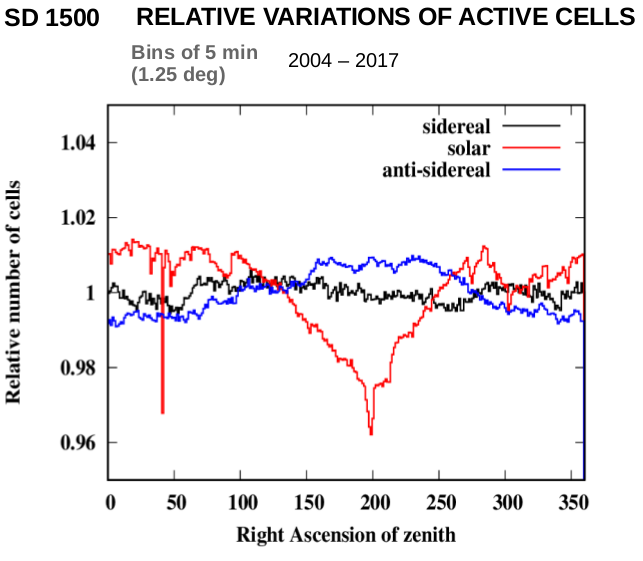
\includegraphics[width=0.8\linewidth]{pesos_referencia.png}  
              \caption{Valores de $\Delta N_{cell, k}$ en el rango 2004-2017 para distintas frecuencias obtenidas en el trabajo \cite{referencia_pesos}.}
              \label{fig:pesos_referencia}
        \end{figure}

       En la Fig.\ref{fig:pesos_ejemplo} se observa valores obtenidos de $\Delta N_{cell,k}$ en función de la ascensión recta del cenit  para $L=288$ segmentos con el programa escrito para este informe, utilizando el mismo conjunto de datos que el utilizado para obtener los resultados la Fig.\ref{fig:pesos_referencia} desde el 1 de Enero del 2004 a las $00:00:00\,$hrs GMT  hasta el 1 de Enero del 2017 a las $00:00:00\,$hrs GMT. Se  observa que estos los resultados obtenidos son compatibles con la Fig.\ref{fig:pesos_referencia}
 

       \begin{figure}[H]
          \centering
              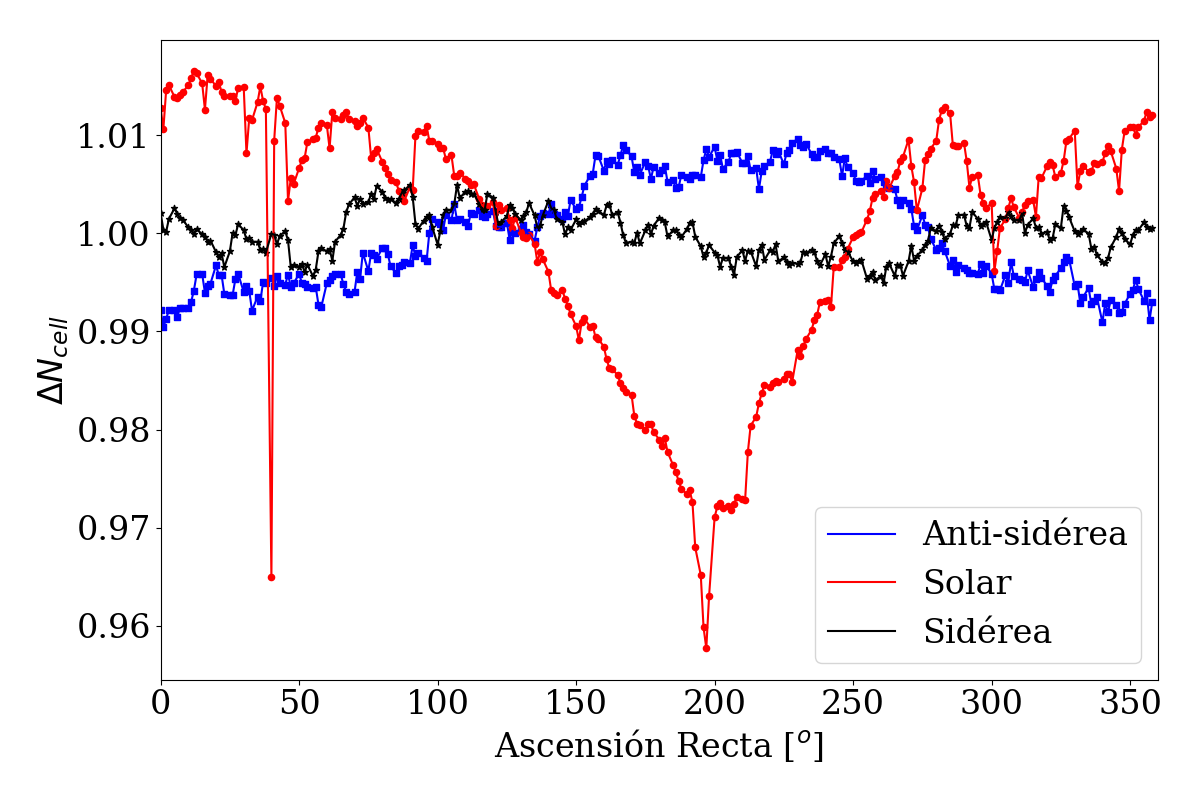
\includegraphics[width=0.8\linewidth]{weigths_2020.png}
              \caption{Valores de $\Delta N_{cell, k}$ en el rango 2004-2017 para distintas frecuencias utilizando el código escrito en este trabajo.}
              \label{fig:pesos_ejemplo}
        \end{figure}


%%%%%%%%%%%%%%%%%%%%%%%%%%%%%%%%%%%%%%%%%%%%%%%%%%%%%%%%%%%%%%%%%%%%%%%%%%%%%%%%%%%%%%%%%%%%%%%%%%%%%%%%%%%%%%%%%%%%%%%%%%%%%%%%%%%%%%%%%%%%%%%%%%%%%%%%%%%%%%%%%%%%%%%%%%%%%%%%%%%%%%%%%%%%%%%%%%%%%%%%%%%%%%%%%%%%%%%%%%%%%%%%%%%%%%%%

  \subsection{Cálculo de Rayleigh para una frecuencia dada} \label{rayleigh}

        \begin{enumerate}
        \item Fijando un rango de tiempo y un rango de energía en el cual se desea estudiar la anisotropía, se establece una frecuencia en particular $f$ a analizar.

        \item Con los eventos ya filtrados según el criterio de la sección \ref{filtro}, asigno cada evento $i$ un valor $h_i$, definida en la Ec.\ref{eq:h_horas}

        \item Para asignar el peso correspondiente al evento, se asocia a un segmento $k$, calculado en la sección \ref{peso_hexagonos}, mediante el valor de $h'_i$ definido en la Ec.\,\ref{eq:h_primado}. Luego, el peso asignado $w_i$  al evento $i$ es
        \begin{equation*}
           w_{i}= (\Delta N_{cell,k})^{-1}
        \end{equation*} 
         
        \item Para el análisis en frecuencias, a partir del valor de $h_i$ se asigna un ángulo $\tilde{\alpha}_i$ como:
        \begin{equation}
         \tilde{\alpha}_i = 2\pi \frac{h}{24} + \alpha_i -\alpha_{cenit,i}
        \end{equation}
        donde $\alpha_i$  representa la ascensión recta del evento y $\alpha_{cenit,i}$ la ascensión recta en el cenit del observatorio en el momento del evento. A partir de este ángulo $\tilde{\alpha}_i$ se realiza en análisis en frecuencias.

        \item Para calcular los coeficientes de Fourier del primer armónico $a$ y $b$, se siguen los siguiente pasos:
        \begin{enumerate}
          \item Por cada evento  $i$ se calculan los siguientes valores:
          \begin{align}
             a_i' = {w_i}\cos\tilde{\alpha}_i \qquad
             b_i' = {w_i}\sin\tilde{\alpha}_i
         \end{align}
         \item Una vez que se obtuvieron los valores de $a_i'$ y $b_i'$ para todos los eventos en el rango de tiempo estudiado, se calculan los coeficientes mediante:
         \begin{alignat}{3}
          \mathcal{N} &= \sum^{Eventos}_i w_i \\
            a &= \frac{2}{\mathcal{N}} \sum^{Eventos}_i a_i' \qquad
            b = \frac{2}{\mathcal{N}} \sum^{Eventos}_i b_i'  
         \end{alignat}
        \end{enumerate}
        \item Con los coeficientes es posible calcular la amplitud de la frecuencia estudiada $\tilde{r}$ y la fase $\phi$. Otros parámetros calculados para el análisis son la probabilidad $P(\tilde{r})$ de que la amplitud obtenida sea producto de una variación de ruido, y el valor de amplitud $r_{99}$ para que dicha probabilidad sea del $1$\%. 
        \begin{alignat}{3}
            \tilde{r} &= \sqrt{a^2 +b^2}             
               \qquad &&   \phi&&= \arctan\frac{a}{b}\\
          P(\tilde{r})&= \exp(-\mathcal{N}\frac{\tilde{r}^2}{4}) 
             \qquad &&   r_{99}&&= \sqrt{\frac{-4\log(0.01)}{\mathcal{N}}}
        \end{alignat}

      \end{enumerate}

    Una forma de validar el código para el análisis de anisotropía es comparar los resultados del código con los obtenidos en otros trabajos \cite{taborda}. En la Fig.\ref{fig:sin_pesos_referencia} se muestra el análisis hecho sobre el mismo conjunto de eventos. Estos eventos fueron adquiridos con el disparo estándar desde el 1 de Enero del 2004 a las $00:00:00\,$GMT  hasta el 1 de Enero del 2017 a las $00:00:00\,$GMT. Se consideraron los eventos por encima de $8\,$EeV que además cumplan las condiciones dadas en la sección \ref{filtro}.  En esta figura que los resultados obtenidos en \cite{taborda} y con el código utilizado por este trabajo son indistinguibles. 

      \begin{figure}[H]
        \centering
        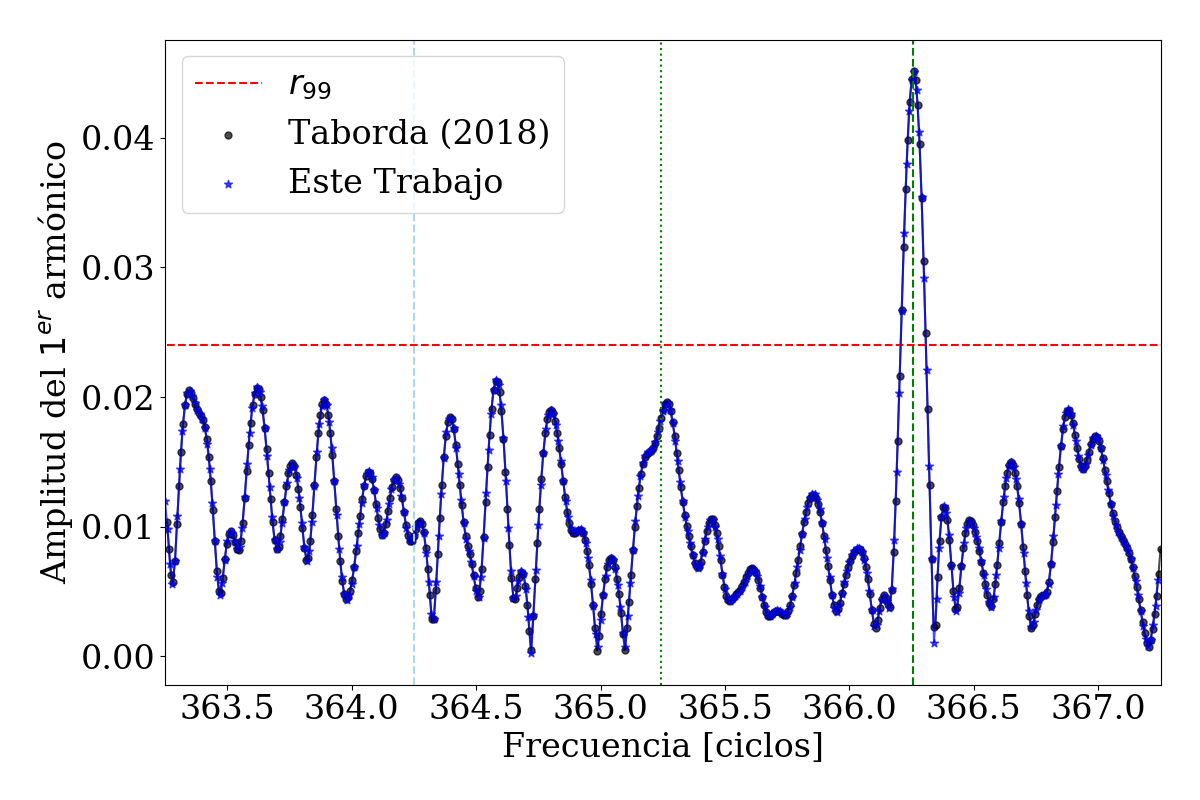
\includegraphics[width=0.75\linewidth]{sin_pesos_referencia_8_EeV.png}
        \caption{Comparación entre los análisis de anisotropía hechos para el mismo conjunto de datos, con el código de \cite{taborda} y con el código escrito para este trabajo.}
        \label{fig:sin_pesos_referencia}
      \end{figure}

% \chapter{Report \#1: 13/04/2020 - Pesos de los hexágonos}
% \graphicspath{{report_1_13_04_2020/}}
% 
\section{Dudas sobre los pesos}

Los pesos de los hexágonos son importantes para el cálculo de anisotropías, porque las anisotropías son pequeñas y eliminar todo factor espúreo es importante.

¿Por qué me trabé tanto? Cuando uso sólo 24 bines, los números entre el paper del 2018 y los que obtengo con mi código son parecidos. En cambio cuando otro bineado, como 360 bines, con el mismo código, hay una diferencia entre lo que se obtiene en el paper mencionado y el mi tesis.

¿Por qué creo que está pasando esto? Si el código funciona para 24 bines, como se muestra en la Fig.\,\ref{fig:all_24}, y cuando sólo cambio la cantidad de bines, como en las Fig.\,\ref{fig:sid_360} y \ref{fig:anti_360}, se ve que sigue la misma tendencia pero no los mismos números. Yo lo que yo creo es que tiene que ver con la precisión del cálculo. Para calcular cada punto, se realiza una división entre dos números, i.e. 
\begin{equation}
	\Delta N = \frac{\text{Los hexágonos integrados en un bin}}{\text{Todos los hexágonos integrados para cada bin}}
\end{equation}


\begin{figure}[H]
	\centering
	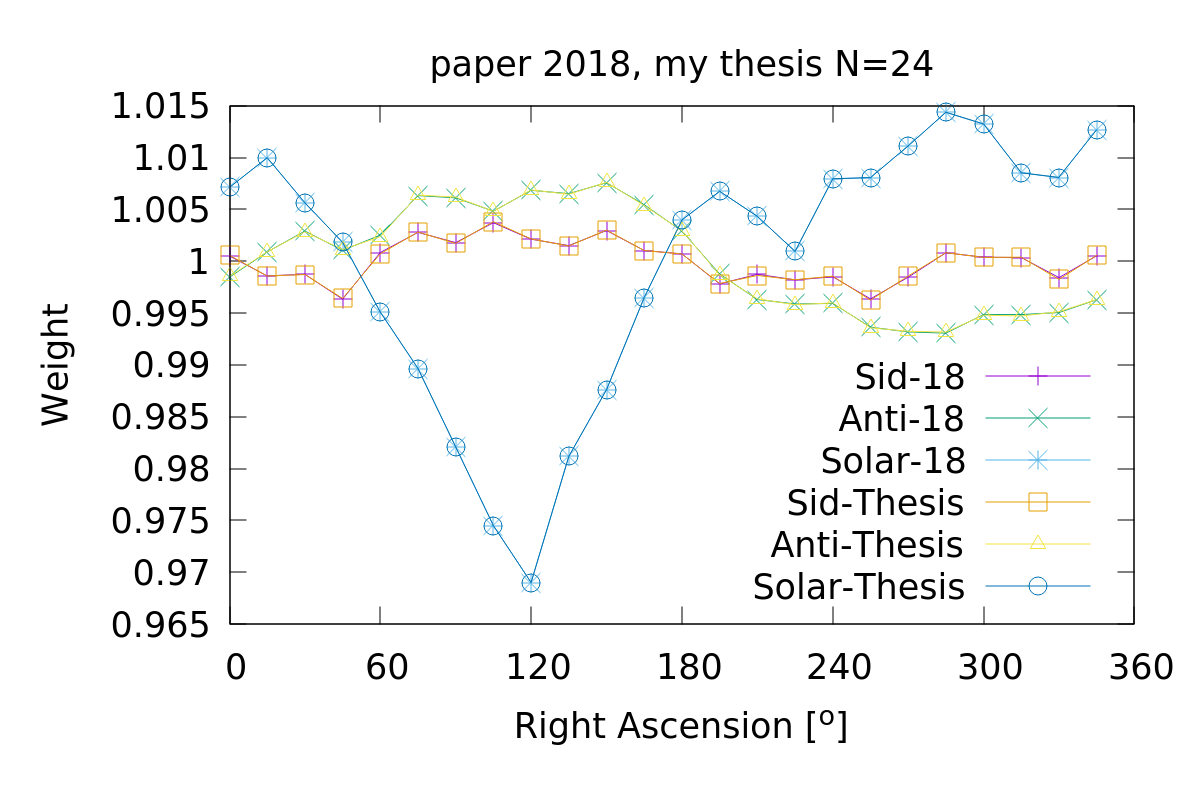
\includegraphics[width=0.45\textwidth]{Graficos/solar_anti_sid_my_and_paper_in_24.png}
	\caption{Usando 24 bines para las frecuencias sidérea, anti-sidérea y solar, se compara el paper del 2018 con lo que obtengo en la tesis.}
	\label{fig:all_24}
\end{figure}


En el caso de $N=24$, son dos números grandes, por lo tanto solo importan los primeros número a izquierda, pero para  $N=360$ es como menor. Durante la ejecución del programa, para cada valor de utc, se calcula a que bin corresponde esa entrada; verifiqué que el programa del paper y mío fuera iguales a cada paso, y constaté que no había diferencias.

Debido a esto, mi hipótesis es la diferencia entre ambos códigos es por la suma de hexágonos. Lo que me causa ruido de esto es que la diferencia entre los puntos del paper y de mi código, para la frecuencia sidérea,  no es ruido centrado en cero como esperaría que fuera si es un error en la precisión, como se muestra en la Fig.\ref{fig:error_360_sid}, lo que me hace dudar de mi hipótesis. En cambio para la frecuencia anti-sidérea, como se ve en la Fig.\ref{fig:error_360_anti}, el error no tiene ninguna modulación.

\begin{figure}[H]
	\centering
	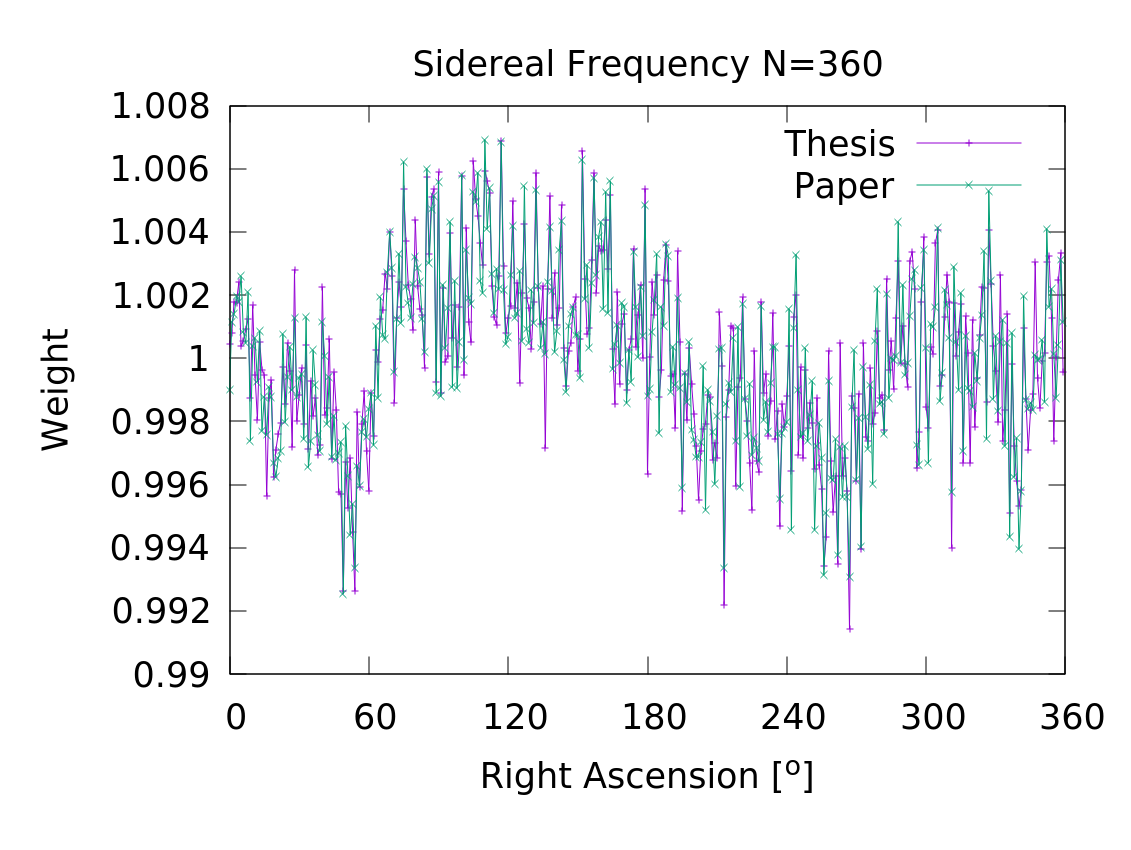
\includegraphics[width=0.45\textwidth]{Graficos/sidereal_my_and_paper_in_360.png}
	\caption{Usando 360 bines para la frecuencia sidérea.}
	\label{fig:sid_360}
\end{figure}


\begin{figure}[H]
	\centering
	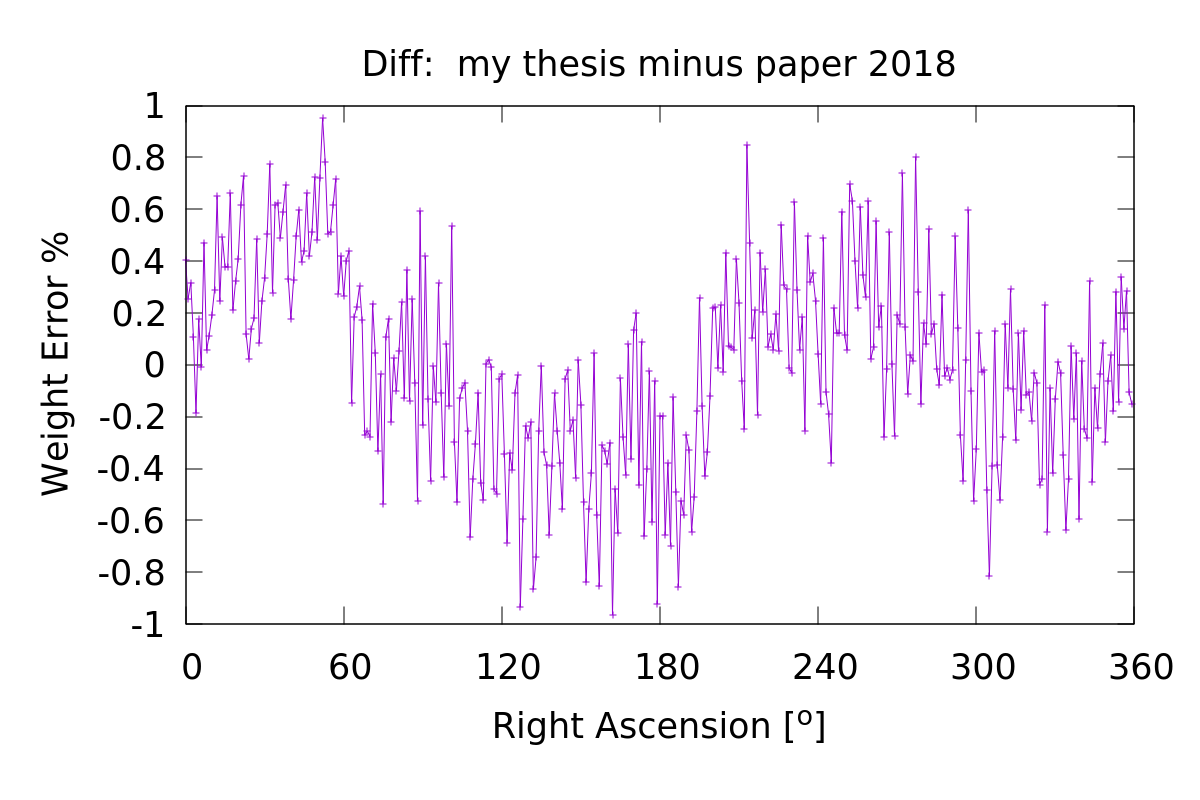
\includegraphics[width=0.45\textwidth]{Graficos/sidereal_my_and_paper_in_360_error.png}
	\caption{Usando los valores del paper como referencia, calculé el error porcentual con lo que yo obtengo para la frecuencia sidérea.}
	\label{fig:error_360_sid}
\end{figure}



\begin{figure}[H]
	\centering
	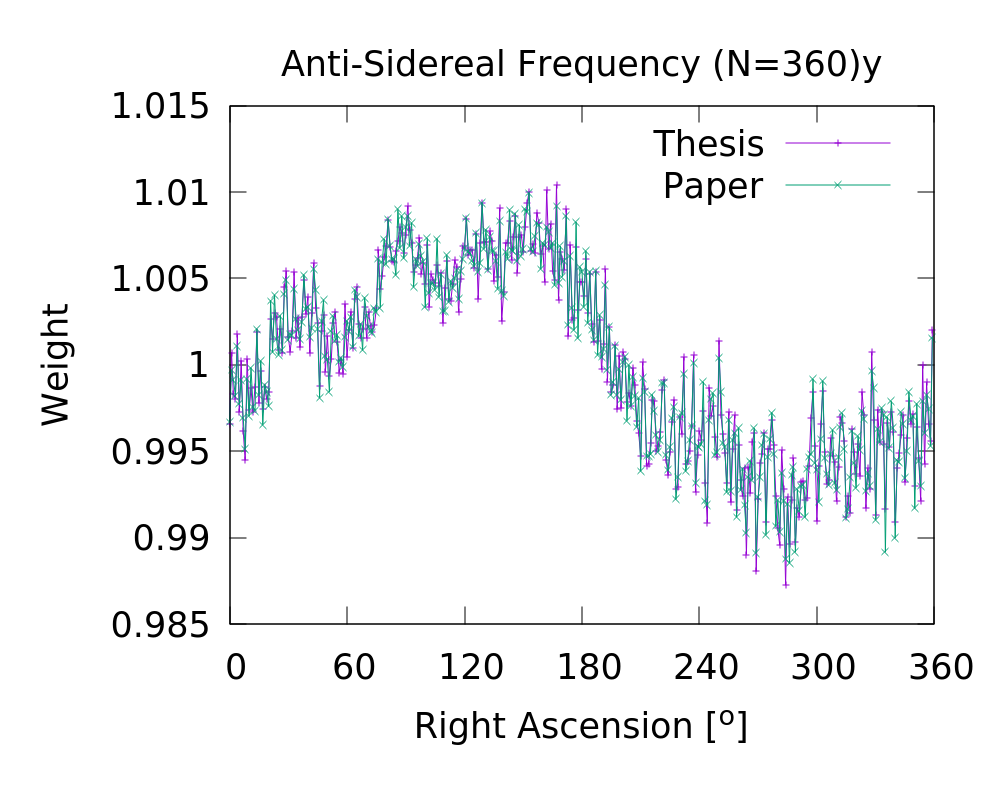
\includegraphics[width=0.45\textwidth]{Graficos/anti_my_and_paper_in_360.png}
	\caption{Usando 360 bines}
	\label{fig:anti_360}
\end{figure}


\begin{figure}[H]
	\centering
	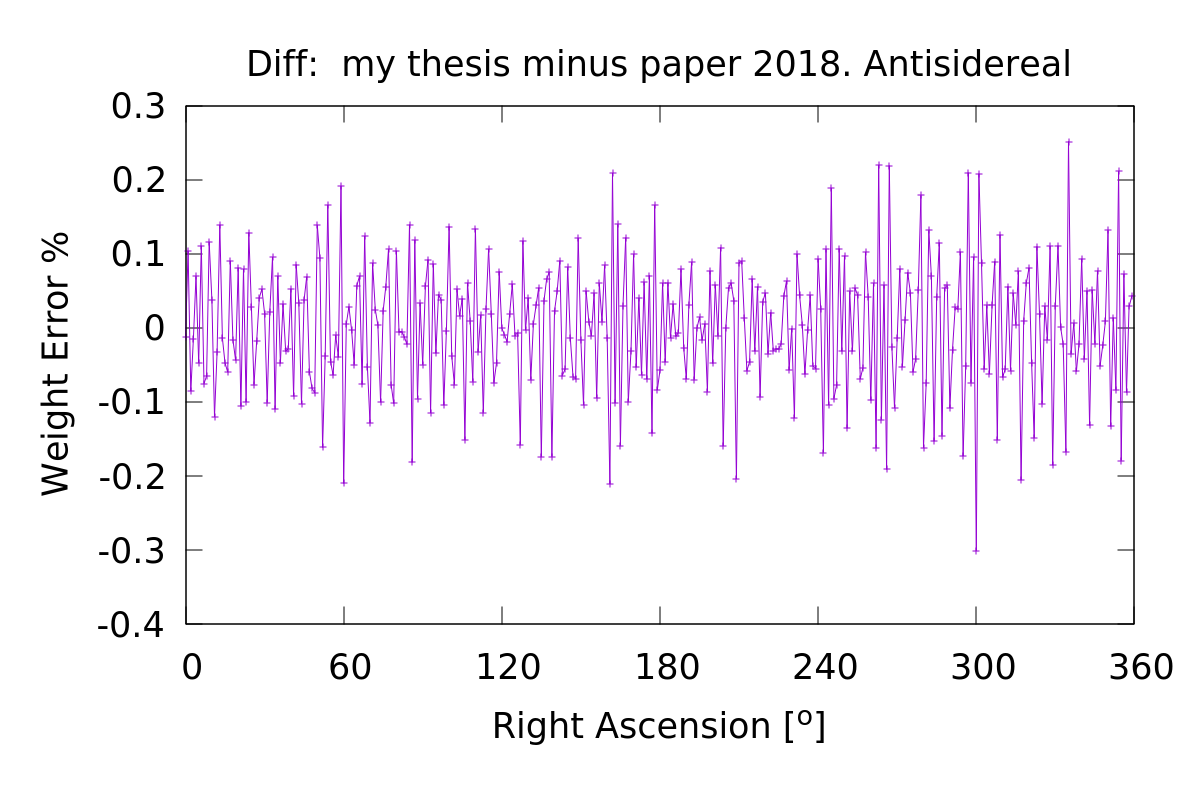
\includegraphics[width=0.45\textwidth]{Graficos/anti_my_and_paper_in_360_error.png}
	\caption{Usando los valores del paper como referencia, calculé el error porcentual de la frecuencia anti-sidérea.}
	\label{fig:error_360_anti}
\end{figure}



\section{Duda sobre los algoritmos}

Contexto: Yo quiero hacer el análisis de los pesos de los hexágonos para distintas frecuencias, por lo que esperaría que para cada frecuencia a analizar se utilice el mismo algoritmo para todos.

Mi duda: En el código del paper 18, el algoritmo hace distinción entre la frecuencia sidérea y las demás. Comparando ambos algoritmos, como se muestra en la Fig.\,\ref{fig:alter_24}, se ve que ambos dan un resultado similar para los pesos de los hexágonos a menos de un desfase de $75^o$ o $5\,$hrs sidéreas. Los gráficos de esta figura se hicieron con el mismo data set.

\begin{figure}[H]
	\centering
	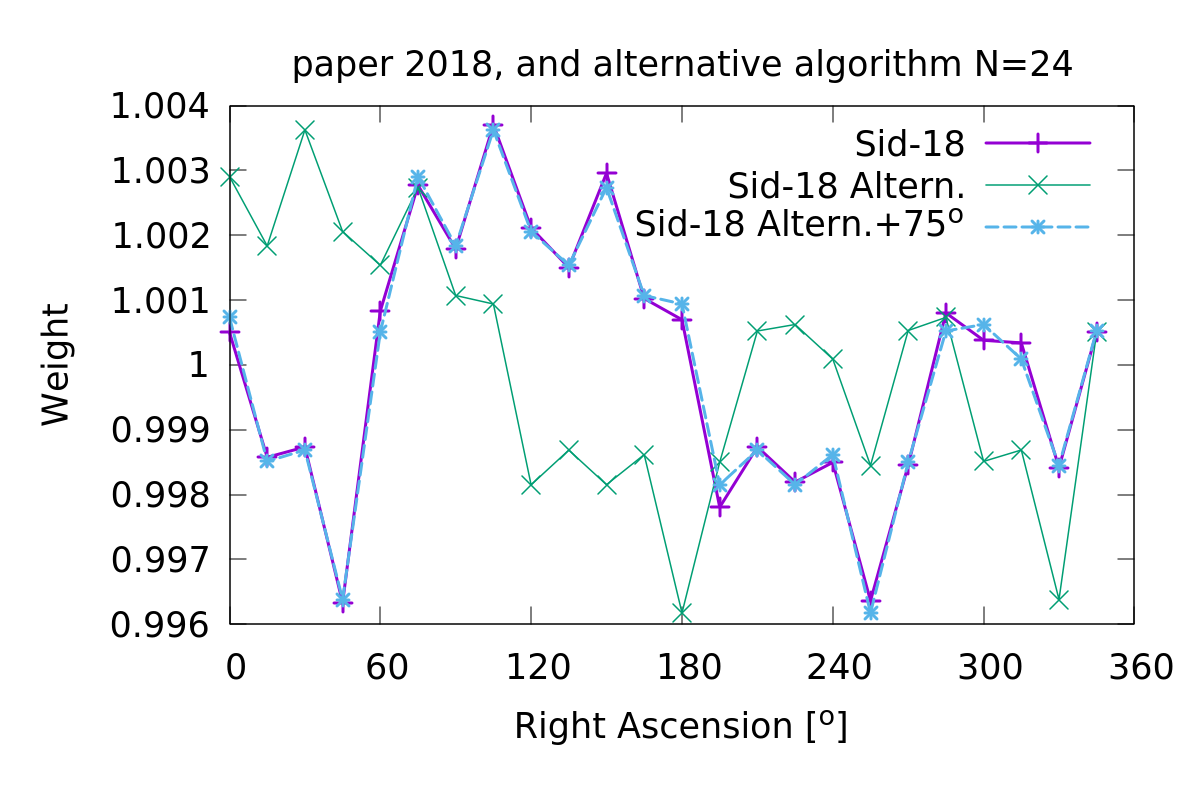
\includegraphics[width=0.45\textwidth]{Graficos/sidereal_paper_in_24_w_alter.png}
	\caption{Comparando el algoritmo alternativo con el utilizado en el paper 18 con resultados del mismo paper, para 24 bines.}
	\label{fig:alter_24}
\end{figure}


Otra cosa que me resultó curiosa fue que usando $N=360$, tengo problemas con la frecuencia solar, donde aparecen 0 cada 5 min, coincide con el rate de actualización del archivo de weather. Así usando este bineado, aparece ese problema, recomendaría no trabajar con bines de $1^o$ en ascensión recta.
\begin{figure}[H]
	\centering
	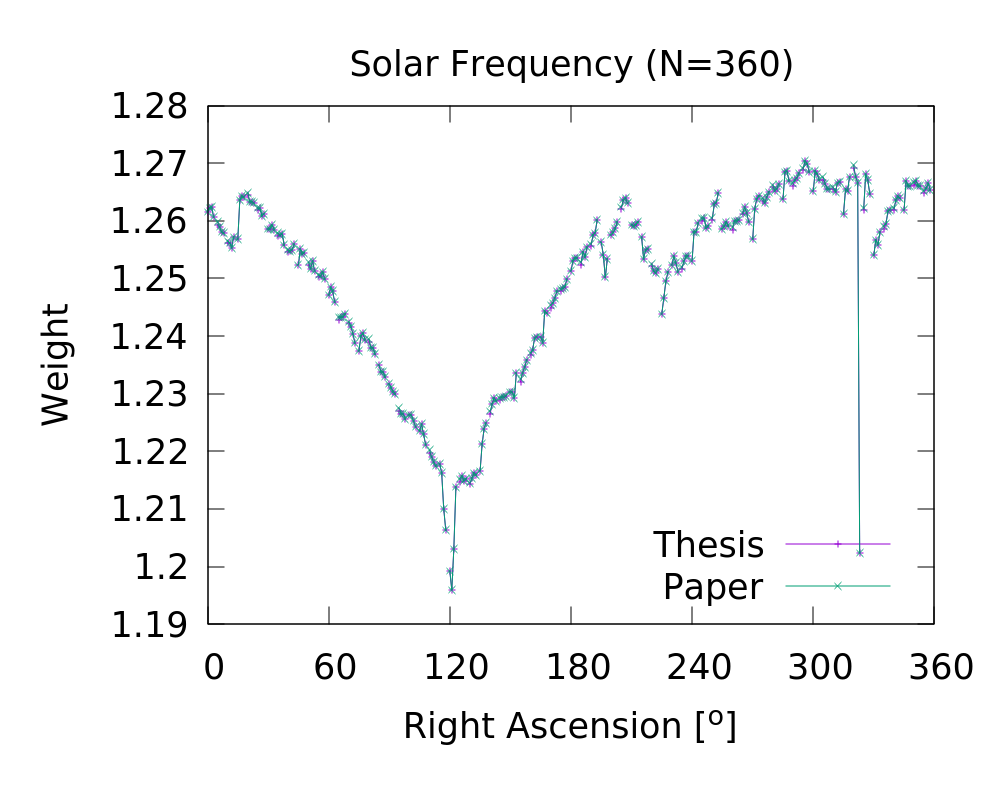
\includegraphics[width=0.45\textwidth]{Graficos/solar_my_and_paper_in_360_2.png}
	\caption{Usando 360 bines, nótese que la media es distinta a la figura anterior.}
	\label{fig:solar_360}
\end{figure}

\section{Para N=288}

El gráfico que me envió usted, sobre los pesos para estas frecuencias es la Fig.\,\ref{fig:all_288_paper}. La discusión sobre estos resultados en particular es análoga al caso para $N=360$, con la diferencia que no tengo valores de anómalos que se ven para la frecuencia solar, Fig.\,\ref{fig:solar_288}.
\begin{figure}[H]
	\centering
	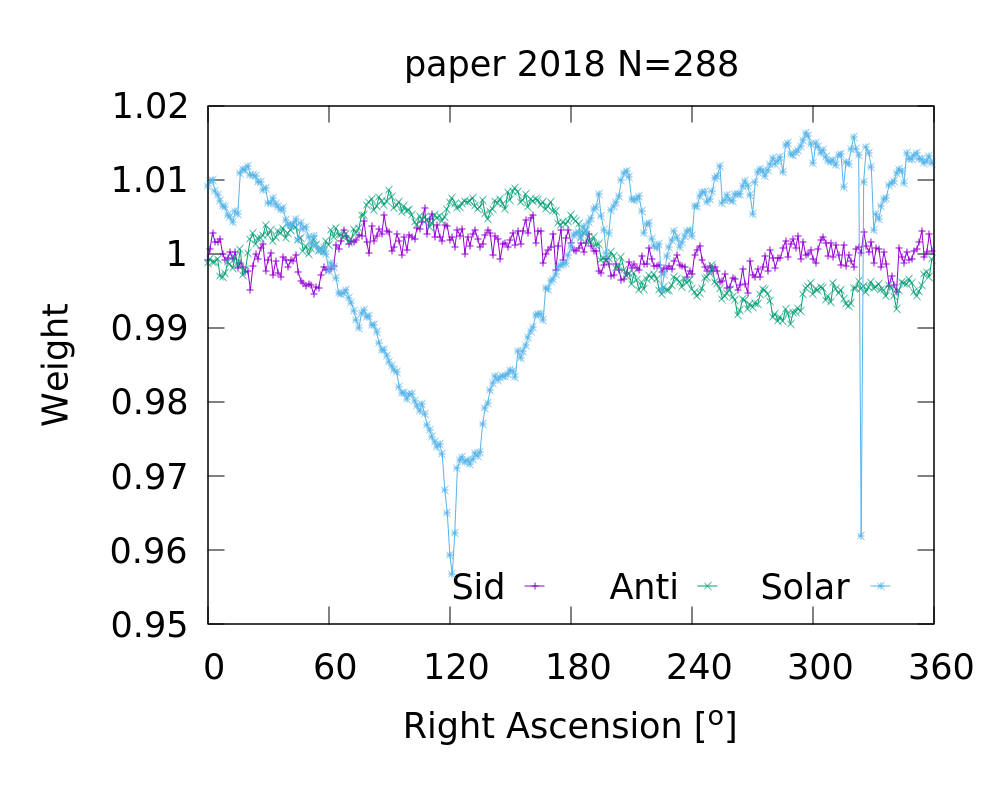
\includegraphics[width=0.45\textwidth]{Graficos/solar_anti_sid_paper2018_in_288.png}
	\caption{Los pesos para las tres frecuencias tal como se calcula en el paper del 2018.}
	\label{fig:all_288_paper}
\end{figure}



\begin{figure}[H]
	\centering
	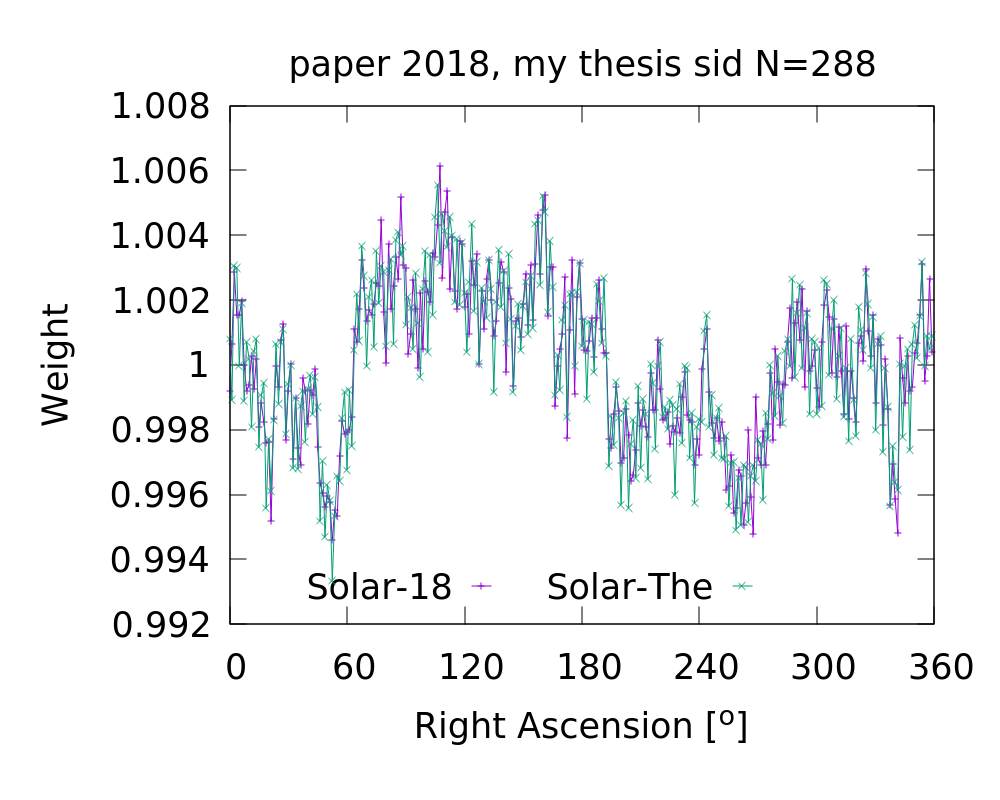
\includegraphics[width=0.45\textwidth]{Graficos/sidereal_my_and_paper_in_288.png}
	\caption{Comparando los resultados del paper con mi código para la frecuencia sidérea para N=288}
	\label{fig:sidereal_288}
\end{figure}


\begin{figure}[H]
	\centering
	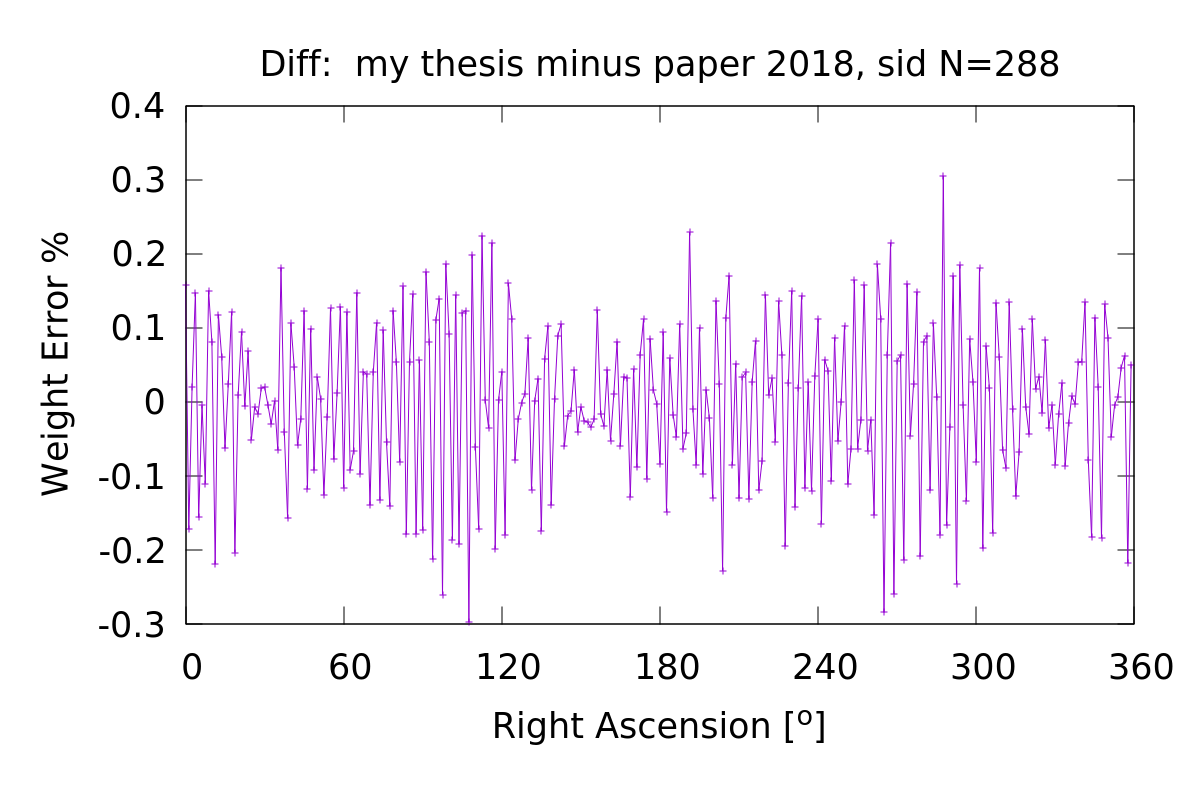
\includegraphics[width=0.45\textwidth]{Graficos/sidereal_my_and_paper_in_288_error.png}
	\caption{El error porcentual entre lo que obtengo en mi código, usando el paper de referencia.}
	\label{fig:error_288_sidereal}
\end{figure}


Ya en la Fig.\,\ref{fig:sidereal_288}, se ve que la media de los pesos es algo razonable comparándolo con N=360, Fig.\ref{fig:solar_360}. Además que el error porcentual, usando como referencia los resultados del paper del 2018, es pequeña. La misma se muestra en la Fig.\,\ref{fig:error_288_solar}.

\begin{figure}[H]
	\centering
	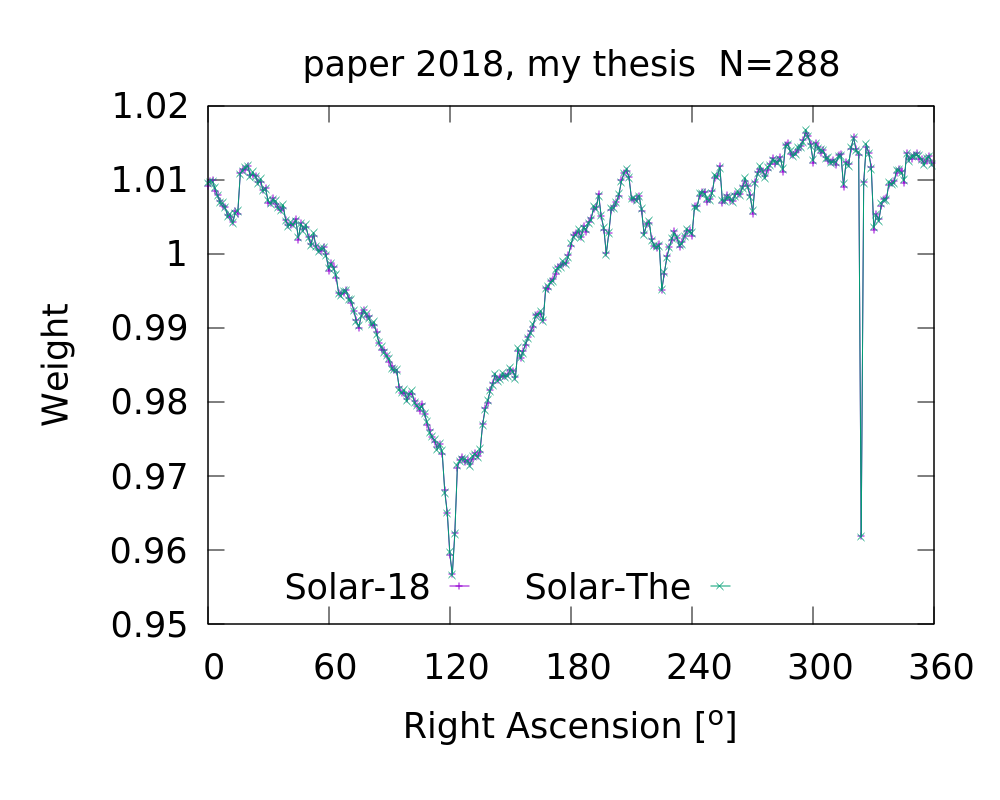
\includegraphics[width=0.45\textwidth]{Graficos/solar_my_and_paper_2018_in_288.png}
	\caption{Pesos para la frecuencia solar.}
	\label{fig:solar_288}
\end{figure}


\begin{figure}[H]
	\centering
	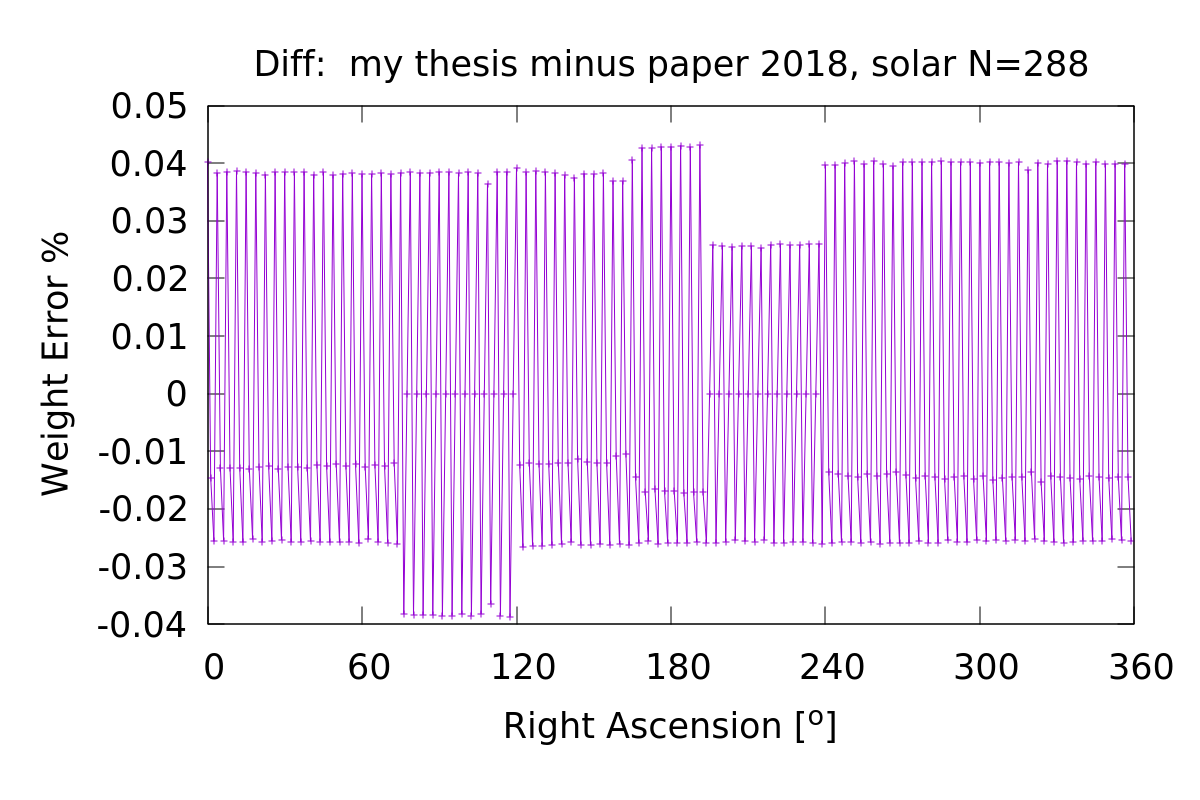
\includegraphics[width=0.45\textwidth]{Graficos/solar_my_and_paper_in_288_error.png}
	\caption{Error porcentual de los pesos de la frecuencia solar con respecto al paper 2018.}
	\label{fig:error_288_solar}
\end{figure}

Para la frecuencia anti-sidérea no hay mucha diferencia a los obtenido para el caso de N=360. Los pesos se muestran en la Fig.\,\ref{fig:anti_288} y el error con respecto al valor del paper se muestra en la Fig.\,\ref{fig:error_288_anti}.

\begin{figure}[H]
	\centering
	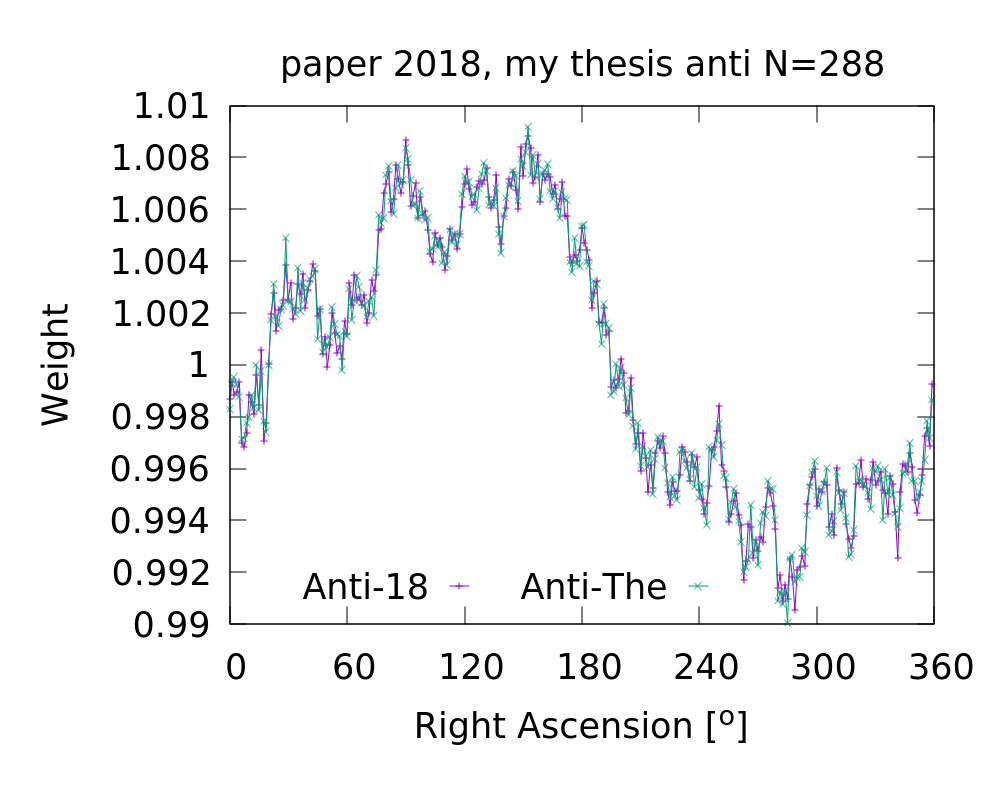
\includegraphics[width=0.45\textwidth]{Graficos/anti_my_and_paper_2018_in_288.png}
	\caption{Pesos para la frecuencia anti-sidérea}
	\label{fig:anti_288}
\end{figure}


\begin{figure}[H]
	\centering
	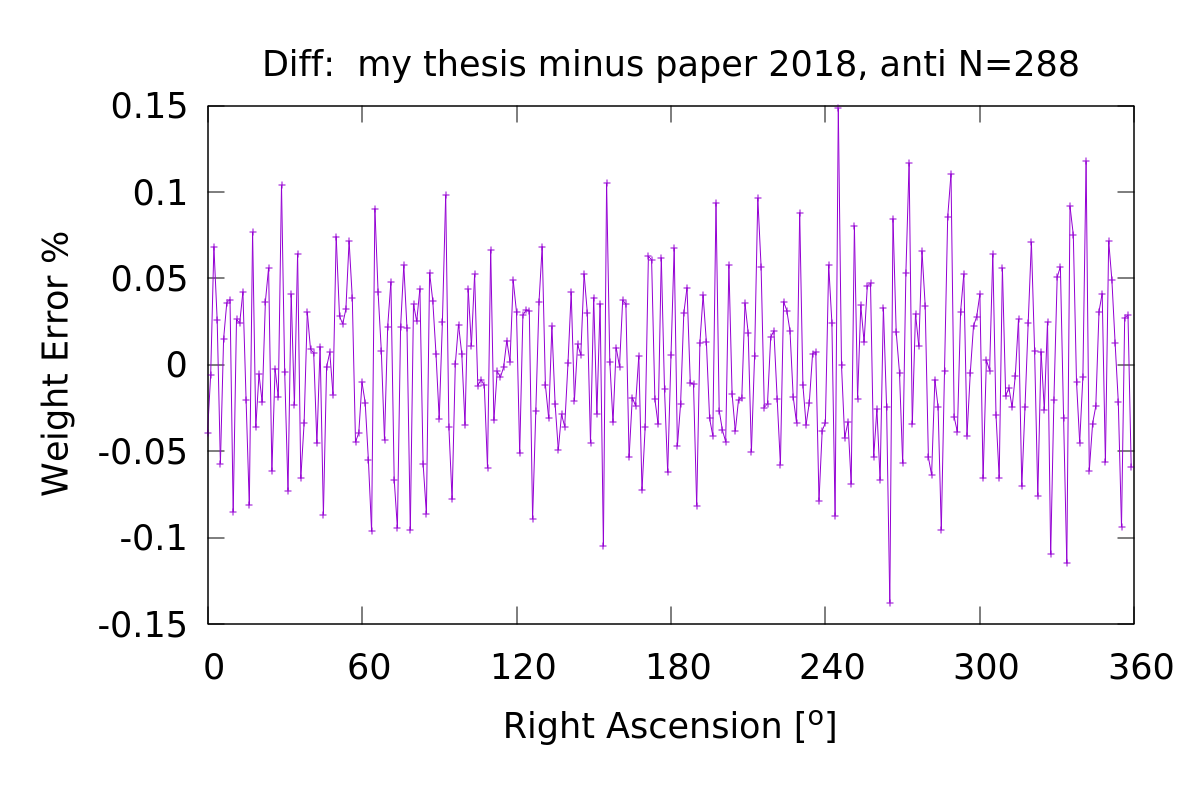
\includegraphics[width=0.45\textwidth]{Graficos/anti_my_and_paper_in_288_error.png}
	\caption{Error porcentual de los pesos de la frecuencia anti-sidérea con respecto al paper 2018.}
	\label{fig:error_288_anti}
\end{figure}


% \chapter{Report \#2: 27/04/2020 - Anisotropías para todos los disparos y pesos de los hexágonos}
% \graphicspath{{report_2_27_04_2020/}}
% %\subsubsection{Nomenclatura}
%ai
%	\begin{table}[H]
%	\centering
%		\begin{tabular}{c|c|c|c}
%	Archivo AllTriggers  & \text{Eventos} & UTC inicial &  UTC final  \\ \hlineaiai
%	2020			 & 13 739 351	  &  1372680068	&  1577879983 \\ %2019
%	2019			 & 	8 463 063	  &	 1372680068 &  1496318388 \\ %Herald
%	2017			 &	8 592 302	  &  1372680068 &  1498521517 \\ %Oscar
%			\end{tabular}
%			\end{table}
%



\section{Anisotropías  considerando el peso de los hexágonos}

\subsection{Verificando que todo funcione como debe}


%Efectos espúreos: Por un lado estan esos piquitos chiquitos, que parecen ser algun problema numerico. Por otro hay todavia demasiados picos arriba de la linea de 99%.


%Se me ocurren dos checks que podrias hacer:

\subsubsection{Comparando con los datos de Oscar}
% 	1-  Uno, que tal vez ya hiciste, es correr tu programa en los datos que uso Oscar y ver de repetir los plots para las dos energias arriba de full efficiency (4-8 y >8)  para ver que el programa funciona igual

\begin{itemize}
	\item Agregar figuras sin peso 
	\begin{itemize}
		\item El de 4-8 para el 2017
		\item >8 para el 2017
	\end{itemize}
	\item buscar los valores de los dipolos conocidos y compararlos con lo que obtengo (usando los pesos)
\end{itemize}

\subsubsection{¿Análisis en frecuencia de los hexágonos?} \label{analisis_peso}
% 	2- Otra prueba que podrias hacer es hacer un  analisis en frecuencia  similar al que hiciste pero para la modulacion de hexagonos sola. Esto seria para ver que no hay cosas raras en el rate de hexagonos de estos datos. No tengo del todo claro como se haria. En vez de hacer la suma de senos y cosenos en los tiempos del zenit cuando llega un evento como ahora, habria que hacer esas sumas en un espaciado constante de tiempo (podrian ser los 5' en que estan bineados, y los pesos deberian ser proporcional a la cantidad de hexagonos. Pensalo un poco como se podria implementar y si queres lo charlamos despues.
\begin{itemize}
	\item ¿Barrido en frecuencia en ascensión recta?
	\item ¿Barriendo el archivo de eventos pero en vez de usar el evento para analizar, uso el valor del peso para el bin correspondiente? Suena bien.
\end{itemize}


%Hola, la fig 1 tiene en solar algunos saltos un poco raros. Podrias hacer esa misma figura (hexagonos en  solar, sidereo y antisidereo) para el periodo de tiempo desde 2004 a dic 2017 (asi comparamos con la comparacion que habian hecho Oscar y Ugo hace un tiempo.
%Y tambien hacela para el periodo completo hasta dic 2019, asi vemos lo que se usa para la ultima parte de tu documento.

\subsubsection{Comparando los pesos en sidérea, solar y antisiderea.}

Un ejemplo de como son los pesos para tres frecuencias en particular, para el rango 2013-2019, se muestra en la Fig.\,\ref{fig:pesos}


\begin{figure}[H]
	\centering
	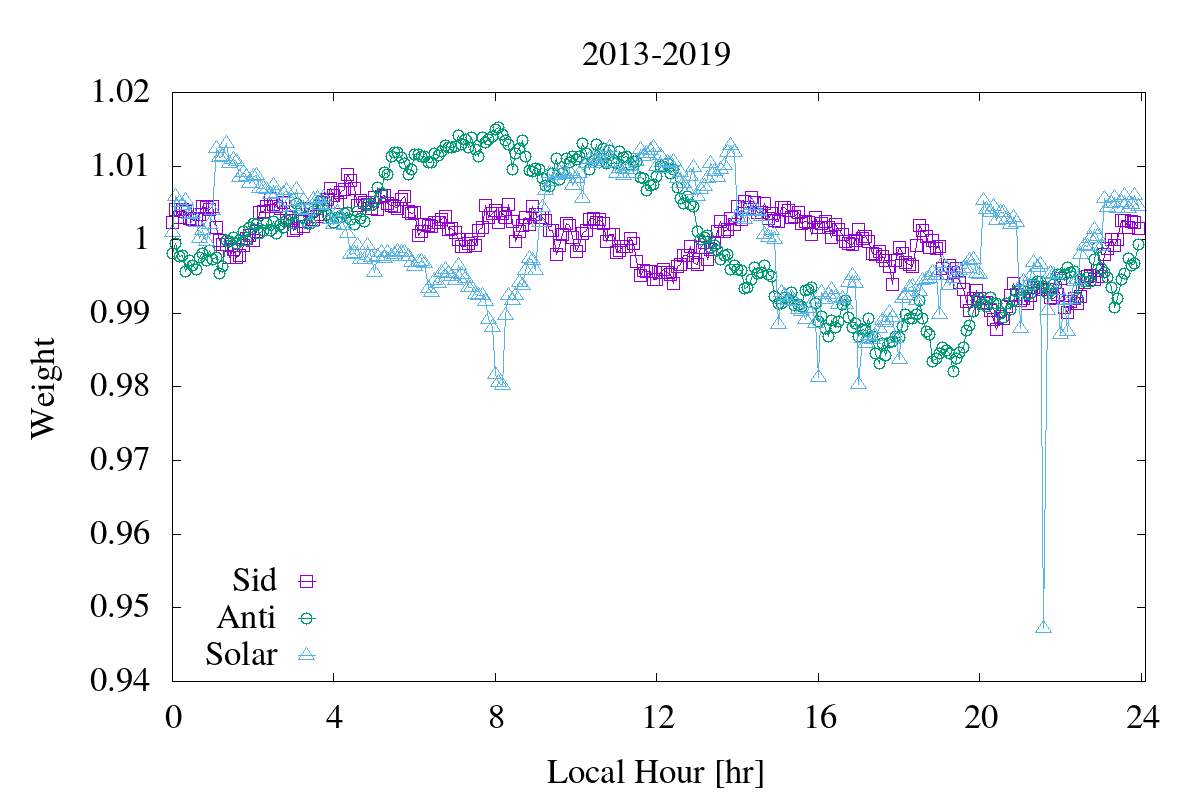
\includegraphics[width=0.5\textwidth]{Graficos/weigth2013-2019.png}
	\caption{Pesos para las frecuencias sidérea, solar y anti-sidérea en el rango 2013-2019}
	\label{fig:pesos}
\end{figure}


Para el rango del 2004 hasta Jun 2017

\begin{figure}[H]
	\centering
	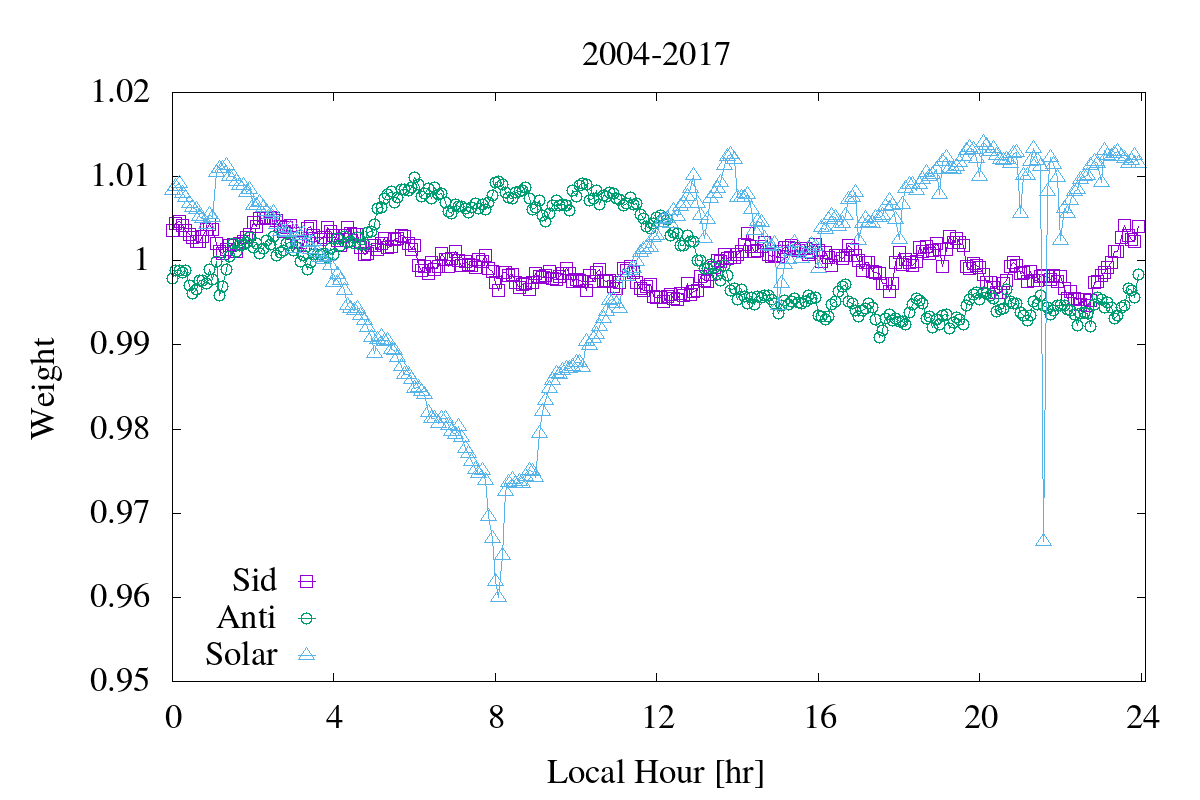
\includegraphics[width=0.5\textwidth]{Graficos/weigth2004-2017.png}
	\caption{Pesos para las frecuencias sidérea, solar y anti-sidérea en el rango 2004-2017}
	\label{fig:pesos_2017}
\end{figure}



Para el rango entre el $2005$ y $2019$
\begin{figure}[H]
	\centering
	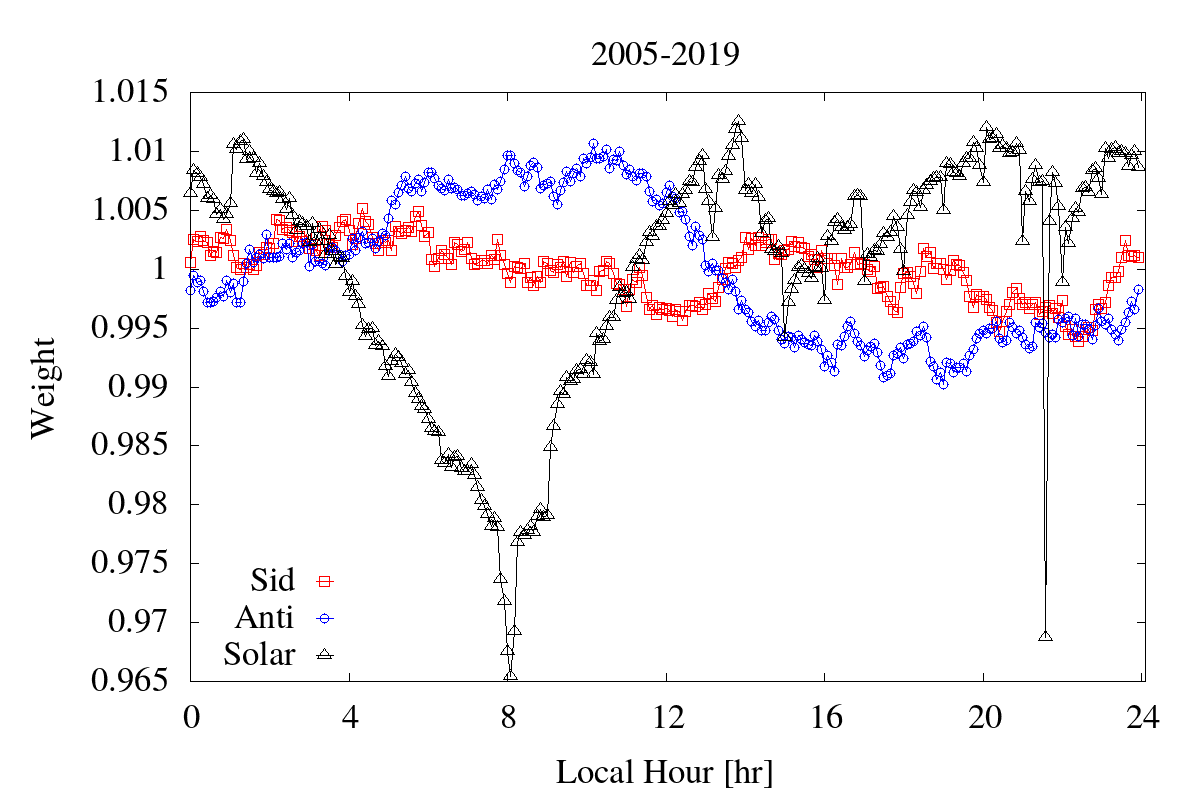
\includegraphics[width=0.5\textwidth]{Graficos/weigth2005-2019.png}
	\caption{Pesos para las frecuencias sidérea, solar y anti-sidérea en el rango 2005-2019}
	\label{fig:pesos_2019}
\end{figure}




La idea que tengo sobre el pico en ambos gráficos es algo en la cantidad de hexagonos, algún periodo donde se apagó la mitad del observatorio o algo así. Quiero hacer la evolución de la cantidad de hexagonos para ese bin en particular en la frecuencia. Estaba pensando en como codearlo para que me sirva también para hacer \ref{analisis_peso}.


%Otra cosa, en general: seria bueno hacer los plots entre 363.25 y 367.25 (ya que las tres que nos interesan son 364.25, 365.25 y 366.25). PARA DESPUÉS
%Otra curiosidad, en frecuencia siderea, cual es la fase en RA y la probabilidad del bin entre 1y 2?


\subsection{Variación de los pesos en función de la ascensión recta}
En las figuras de esta sección se muestran el análisis en ascensión recta para los eventos de observatorio considerando las variaciones de la exposición. 
Los mismos se hicieron en el mismo intervalo de tiempo para poder compararlos entre sí. Elegí el rango presentado en la Tabla \ref{rango_corto}  porque en el mismo se encuentran todos los eventos filtrados por energía, por bad period, por reconstrucción correcta, etc. El rango empieza en el 2013 porque la última versión del archivo de todos los disparos empezó a registrarse desde el  1 de Julio del 2013 a las 12:01:08 GMT (1372680068) hasta el  1 de enero del 2020 a las 11:59:43 (1577879983). Mientras que el archivo del disparo estándar va desde el 01 de enero del 2004.

	\begin{table}[H]
	\centering
		\begin{tabular}{c|c|c|c}
	 		& UTC 			& Fecha		 	&  Hora GMT  \\ \hline
	Inicio	& 1372699409	&2013-07-01 	&17:23:29		\\
	Final 	& 1577825634	&2019-12-31 	&20:53:54		\\
		\end{tabular}
	\caption{Rango de tiempo considerando todos los disparos} 	\label{rango_corto}
	\end{table}


\subsubsection{Energía entre 1\,EeV y 2\,EeV}

Para este caso utilizamos el archivo con todos los disparos en el rango de energía $1\,$ EeV - $2\,$EeV donde se tiene $1\,321\,702$ eventos.

\begin{figure}[H]
	\centering
	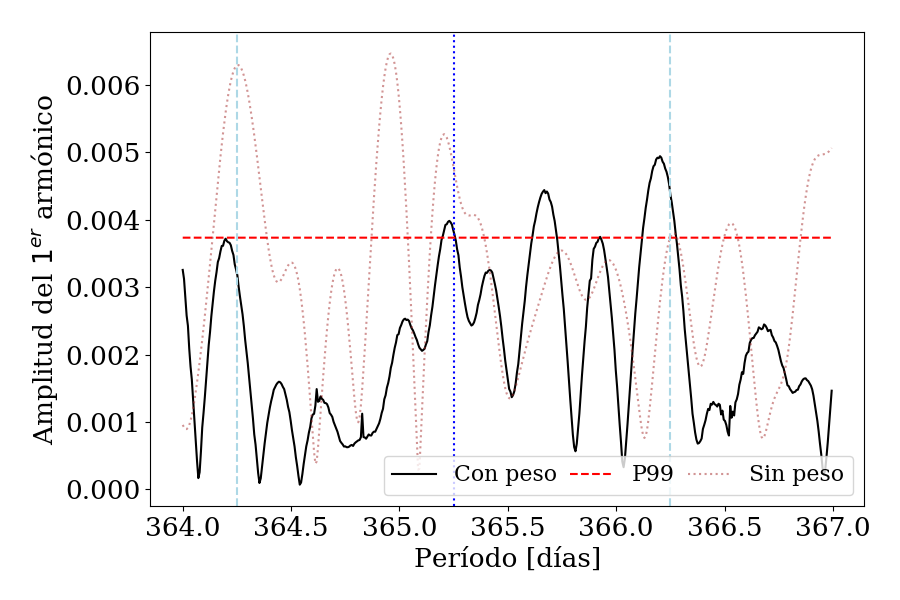
\includegraphics[width=0.5\textwidth]{Graficos/2019_AllTriggers_1_2_EeV_con_vs_sin_peso.png}
	\caption{Todos los disparos: entre 1 EeV y 2 EeV, entre 2013-2019}
	\label{fig:12w}
\end{figure}
%fig

\emph{Otra curiosidad, en frecuencia siderea (366.25), cual es la fase en RA y la probabilidad del bin entre 1y 2?}

La siguiente tabla se había calculado usando la formula 

\begin{equation}
	\tilde \alpha = 2\pi \frac{t_i}{T_x} +\alpha_i - \alpha^0
\end{equation}
donde $\alpha_i$ y $\alpha^o$ con las RA del evento y del cenit del observatorio.

	\begin{table}[H]
	\centering
		\begin{tabular}{c|c}
	 		&  2013-2019 (Con peso)	 \\ \hline
	Fase		& 	306.611				 \\
	$r$ 		&  0.00440897			\\
	$r_{99}$ 	&  0.00373348			\\
	$P(\tilde r)$ 	    & 	0.162485	\%	 \\
		\end{tabular}
	\caption{Rango de tiempo considerando todos los disparos} 	\label{rango_corto}
	\end{table}


\subsubsection{Energía entre 2\,EeV y 4\,EeV}

Para este caso utilizamos los eventos del archivo con todos los disparos con energía entre $2\,$ EeV - $4\,$EeV, donde se encontraron $288\,444$ eventos.
\begin{figure}[H]
	\centering
	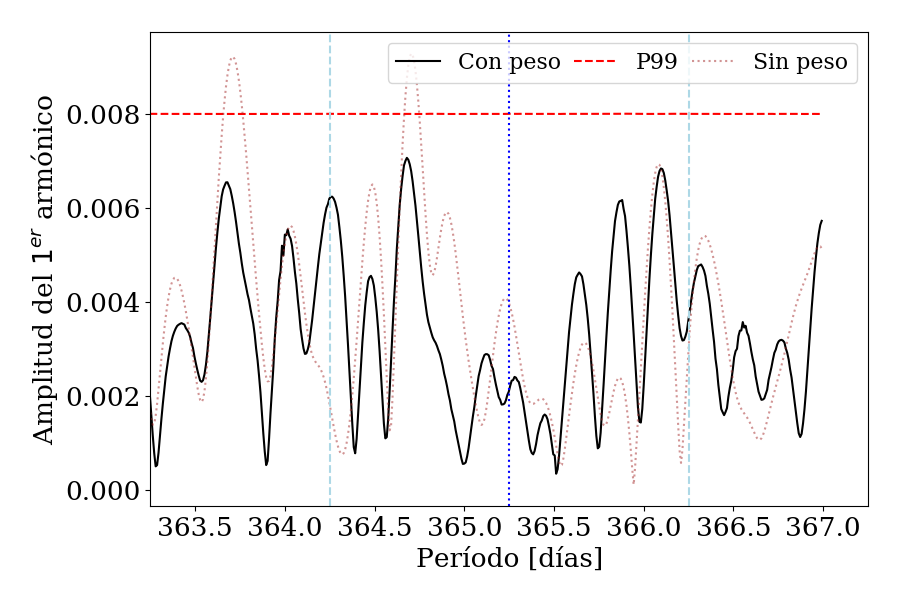
\includegraphics[width=0.5\textwidth]{Graficos/2019_AllTriggers_2_4_EeV_con_vs_sin_peso.png}
	\caption{Todos los disparos: entre 2 EeV y 4 EeV, entre 2013-2019}
	\label{fig:24w}
\end{figure}

En la Fig.\,\ref{fig:24w} no se ve ningún pico por encima de  percentil 99.


\subsubsection{Energía entre 4\,EeV y 8\,EeV}

A partir de $3\,$EeV el disparo estándar tiene una eficiencia del $100\%$. Entonces para este  intervalo de energías,  utilizamos el archivo con el disparo estandar.

\begin{figure}[H]
	\centering
	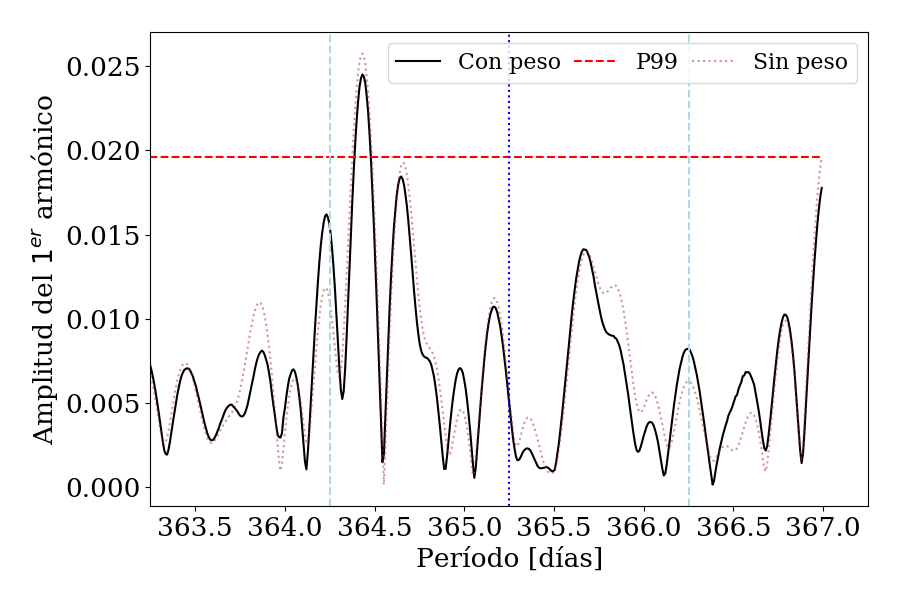
\includegraphics[width=0.5\textwidth]{Graficos/2019_Main_Array_4_8_EeV_con_vs_sin_peso.png}
	\caption{Disparos estándar: entre 4 EeV y 8 EeV, entre 2013-2019}
	\label{fig:48w}
\end{figure}
%fig

\subsubsection{Energía sobre 8\,EeV}

Para este caso utilizamos el archivo con el disparo estandar

\begin{figure}[H]
	\centering
	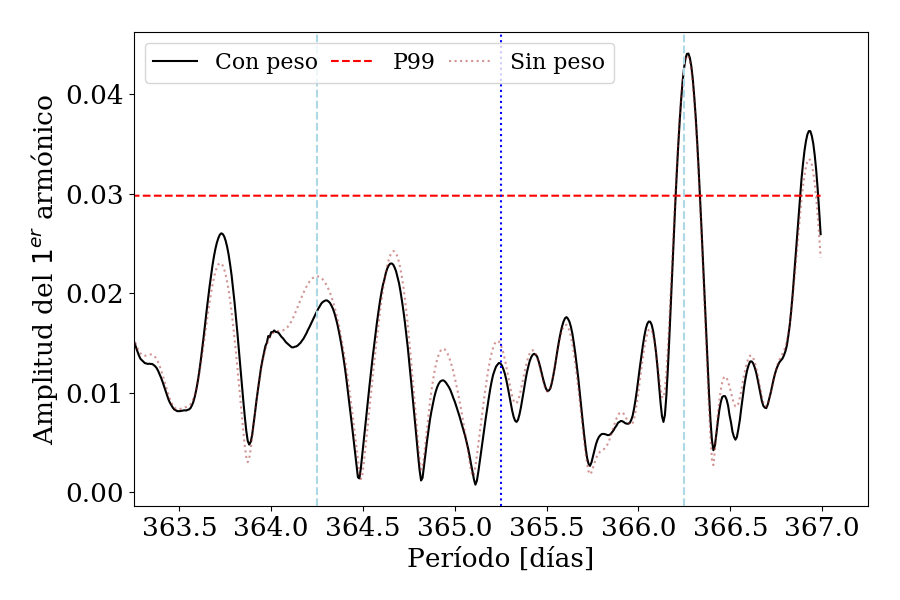
\includegraphics[width=0.5\textwidth]{Graficos/2019_Main_Array_8_EeV_con_vs_sin_peso.png}
	\caption{Disparos estándar: encima de 8 EeV, entre 2013-2019}
	\label{fig:8w}
\end{figure}
%fig




\subsection{Ampliando el rango de tiempo para el archivo del disparo estándar}

Amplié el rango de tiempo para poder compararlo con los gráficos anteriores, ya que se espera que mientras mayor sea el rango de tiempo los efectos espúreos disminuyen.

	\begin{table}[H]
	\centering
		\begin{tabular}{c|c|c|c}
	 		& UTC 			& Fecha		 	&  Hora GMT  \\ \hline
	Inicio	& 1104537600	&2005-01-01 	&00:00:00		\\
	Final 	& 1577825634	&2019-12-31 	&20:53:54		\\
		\end{tabular}
	\end{table}


\subsubsection{Energía entre 4\,EeV y 8\,EeV}

\begin{figure}[H]
	\centering
	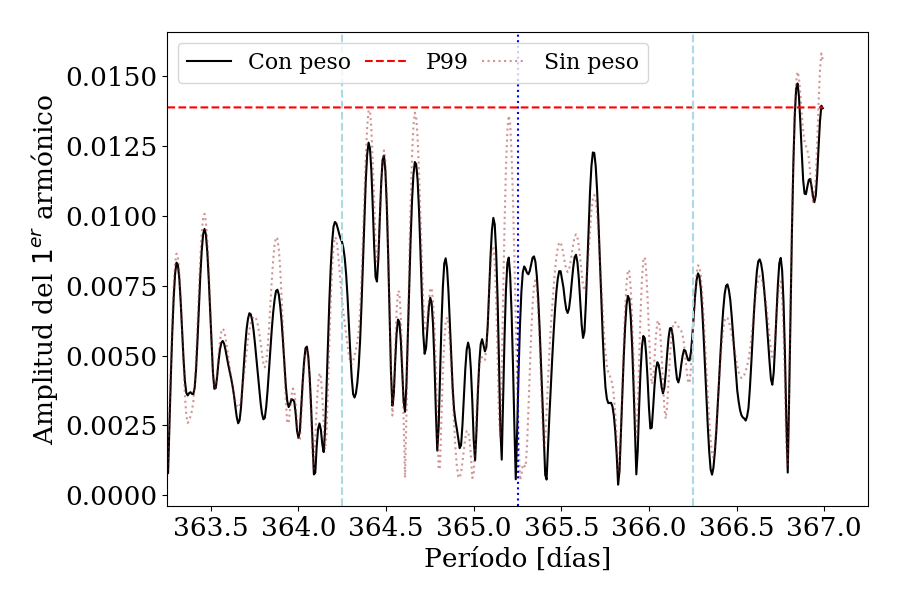
\includegraphics[width=0.5\textwidth]{Graficos/2019_Main_Array_4_8_EeV_con_vs_sin_peso_extended.png}
	\caption{Disparos estándar: entre 4 EeV y 8 EeV extendiendo el rango hasta el 2005}
	\label{fig:48w_extended}
\end{figure}
%fig

\subsubsection{Energía sobre 8\,EeV}


\begin{figure}[H]
	\centering
	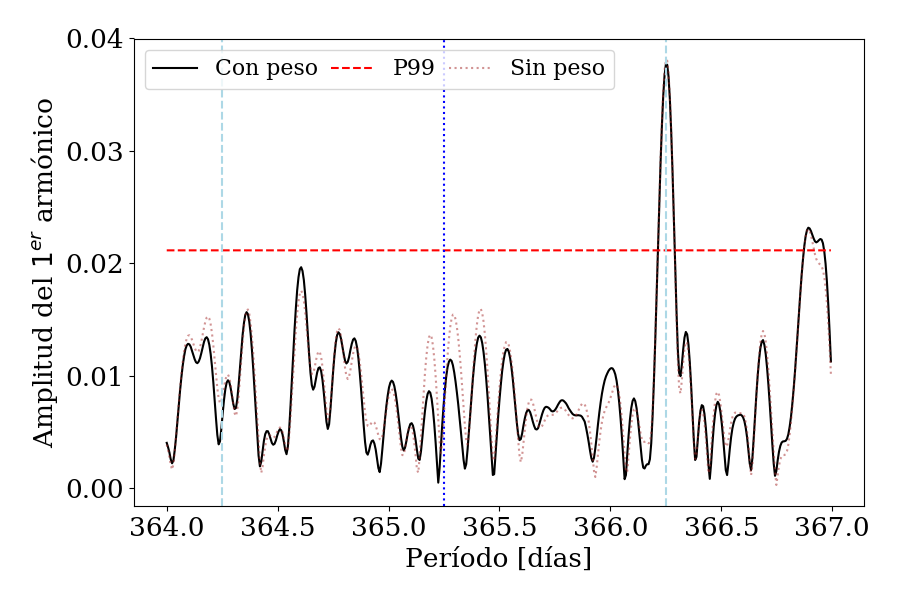
\includegraphics[width=0.5\textwidth]{Graficos/2019_Main_Array_8_EeV_con_vs_sin_peso_extended.png}
	\caption{Disparos estándar: encima de 8 EeV extendiendo el rango hasta el 2005}
	\label{fig:8w_extended}
\end{figure}
%fig

% \chapter{Report \#3: 07/05/2020 - Reconstrucción de energía}
% \graphicspath{{report_3_07_05_2020/}}
% 

\subsection{Rango de tiempo}
\begin{table}[H]
\centering
\begin{tabular}{c|c|c}
Inicio & 1388628499 & 2 January 2014 \\ \hline
Final  & 1550534100 & 18 February 2019 \\
\end{tabular}
\end{table}

\subsection{Tasa de eventos}

\begin{figure}[H]
	\centering
	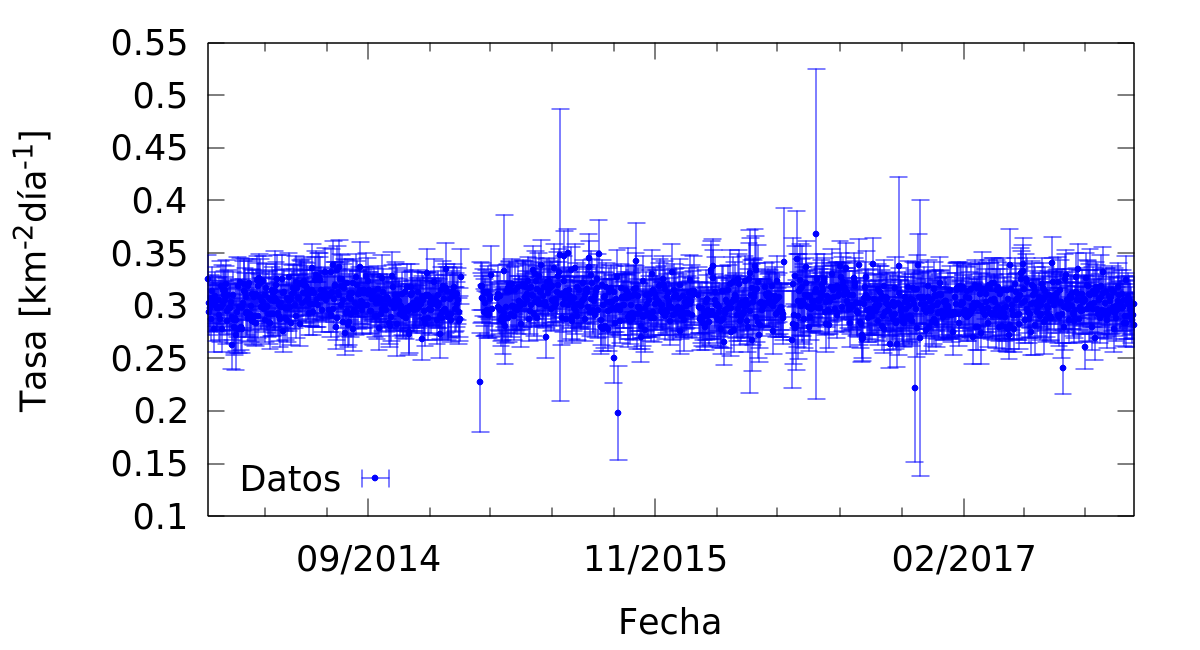
\includegraphics[width=0.5\textwidth]{rate_1_EeV.png}
	\caption{Tasa de eventos para eventos por encima de 1 EeV.}
\end{figure}

Antes del 2 de Enero del 2014, se tenía una tasa por debajo de la media de los siguientes años.

La cantidad de hexágonos 6T5 durante el periodo mencionado arriba evolucionó como se muestra  en la figura que sigue


\begin{figure}[H]
	\centering
	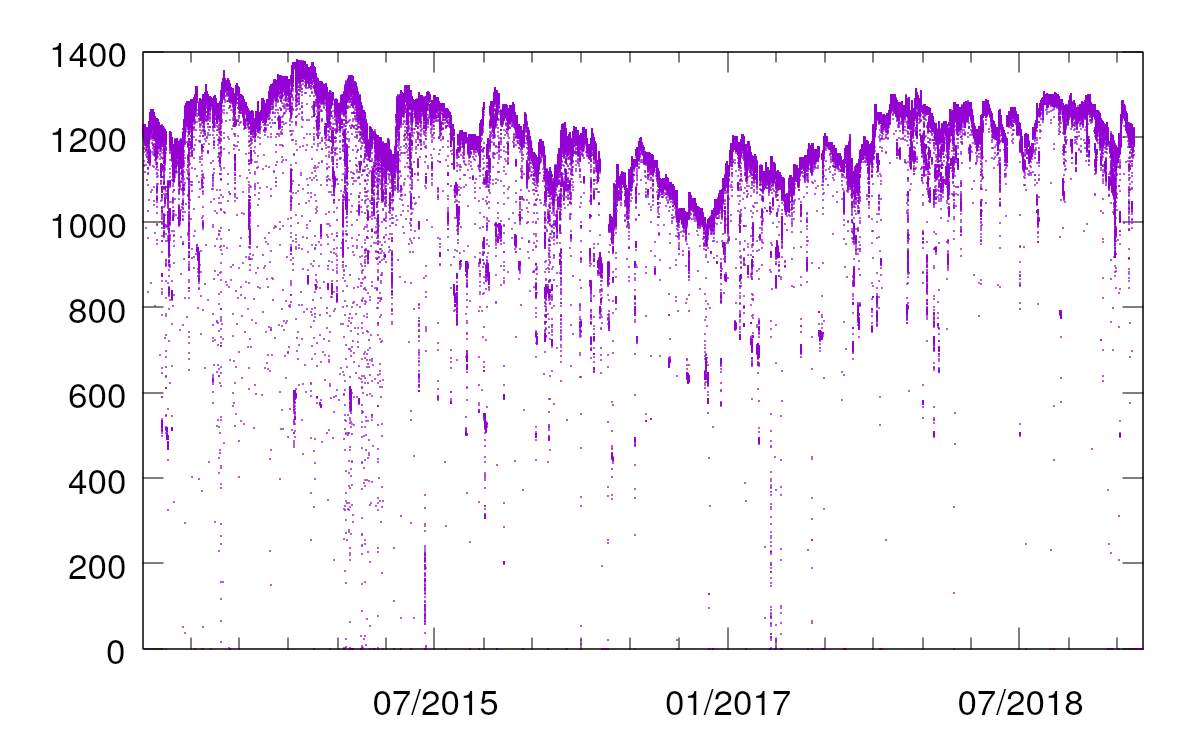
\includegraphics[width=0.5\textwidth]{hex_rango_corto.png}
	\caption{Hexágonos}
\end{figure}


\subsection{Párametros del clima}

\begin{figure}[H]
	\centering
	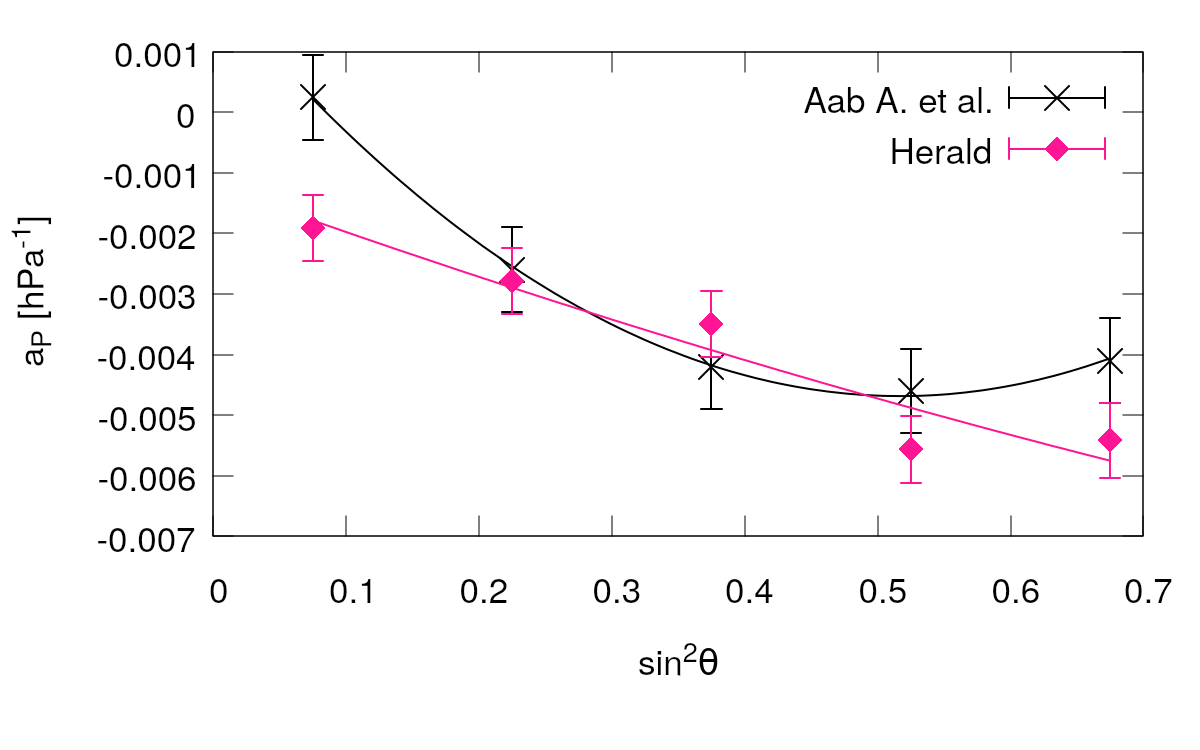
\includegraphics[width=0.5\textwidth]{ap.png}
\end{figure}


\begin{figure}[H]
	\centering
	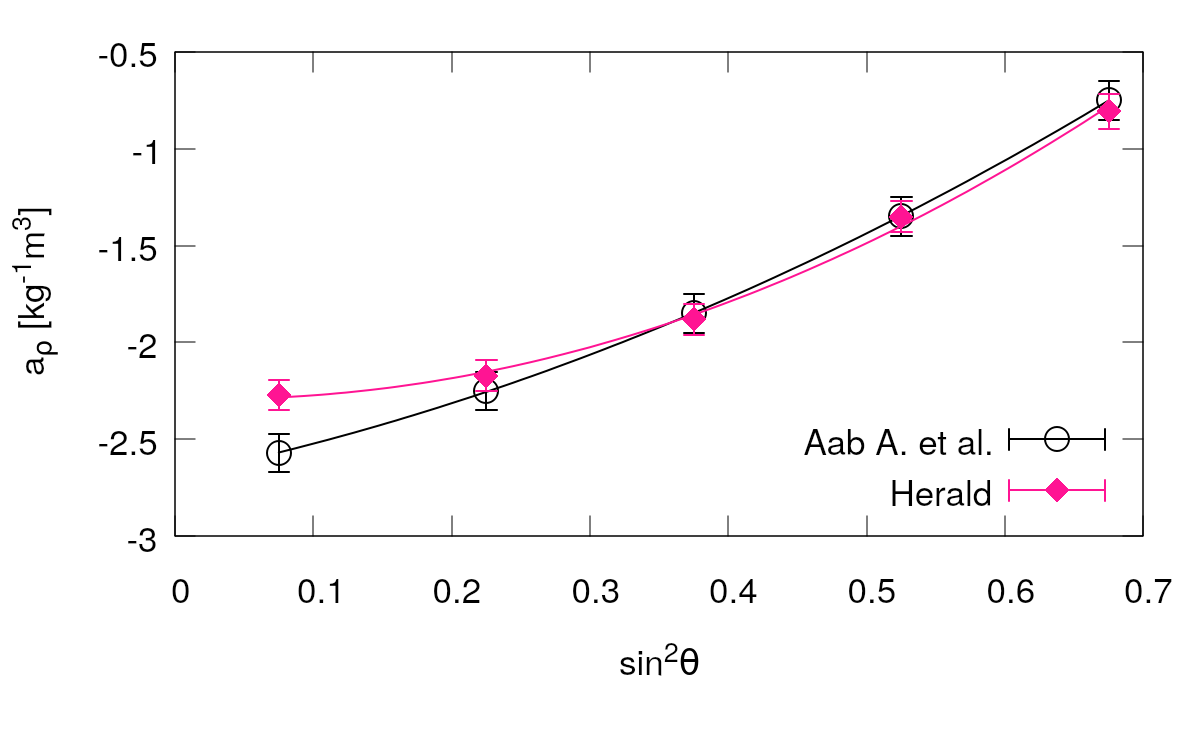
\includegraphics[width=0.5\textwidth]{arho.png}
\end{figure}


\begin{figure}[H]
	\centering
	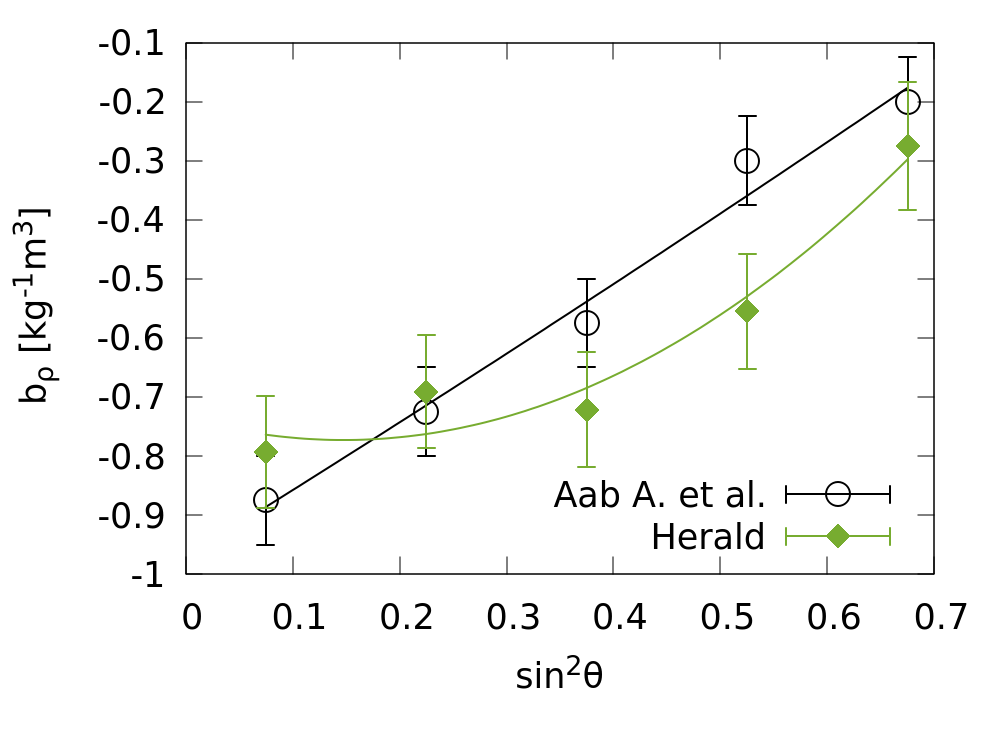
\includegraphics[width=0.5\textwidth]{brho.png}
\end{figure}




Considerando una cuádrica para el ajuste de la curva, se obtiene los parámetros de la siguiente table
\begin{table}[H]
\centering
\begin{tabular}{c|c|c|c}
		 	& $a_P$ 	&  $a_\rho$  & $ b_\rho$ \\ \hline
$c_0$ 		& -0.002(1) & 	-2.2(1)	 &	-0.74(9)\\ \hline
$c_1$ 		& -0.009(6)	& 	 0.4(6)	 &	-0.0(6)\\ \hline
$c_2$ 		&  0.00(9) 	& 	 2.7(8)  &	 1.7(7)\\ \hline
\end{tabular}
\end{table}


\subsection{Anisotropía en el rango 1-2 EeV}

\begin{figure}[htbp]
	\centering
	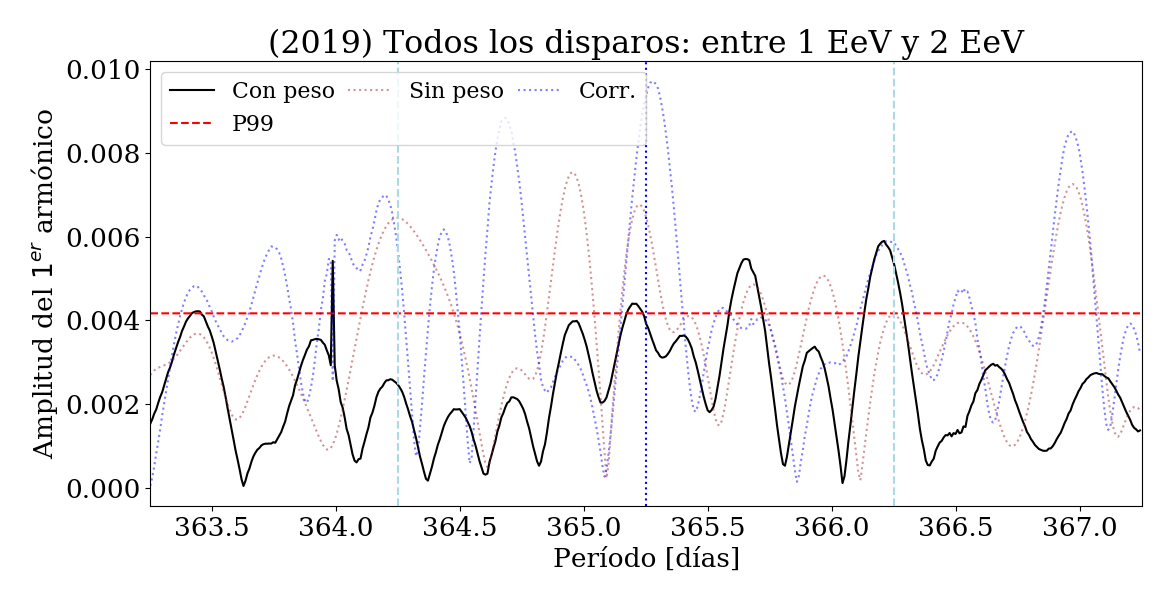
\includegraphics[width=0.5\textwidth]{ani_corr.png}
\end{figure}


\chapter{Modulación del clima para todos los disparos (2014-2020)}
\graphicspath{{report_4_12_05_2020/}}

La selección de los eventos genera dos conjuntos de datos: uno para el análisis de anisotropía en el bin 1 EeV - 2 EeV, y el segundo de los eventos con energía mayor a 1 Eev para obtener los parámetros del clima. En esta selección se tiene en cuentan los eventos de $\theta < 60^o$ \footnote{el archivo que bajo de \url{http://ipnwww.in2p3.fr/~augers/AugerProtected/herald.php} }, como también  los mismos que no se encuentren en un periodo de mala adquisición datos, este parámetro se denomina $ib$ de los \textbf{eventos del herald}. Este periodo consiste en momento donde el obsevatorio no recibe datos de las estaciones de clima o de los hexágonos. 

El parámetro de $ib$ de los \textbf{datos del clima} es irrelevante durante el proceso de filtrar eventos. Entra en juego cuando hago el análisis del clima, donde desecho los eventos que fueron recabados durante \emph{bad weather} \textbf{y} no fueron filtrados ya antes. 


\section{Pesos de los hexágonos}

Para constatar que no exista ninguna anomalía en los pesos de los hexágonos, se realiza el cálculo de los mismos para tres frecuencias de referencia para el análisis de anisotropías.  Los pesos se muestran en la Fig.\,\ref{fig:wei_14_20}. El rango de tiempo en el que se calculan estas curvas es entre 1 de Enero del 2014 y el 1 de Enero del 2020.

\begin{figure}[H]
	\centering
	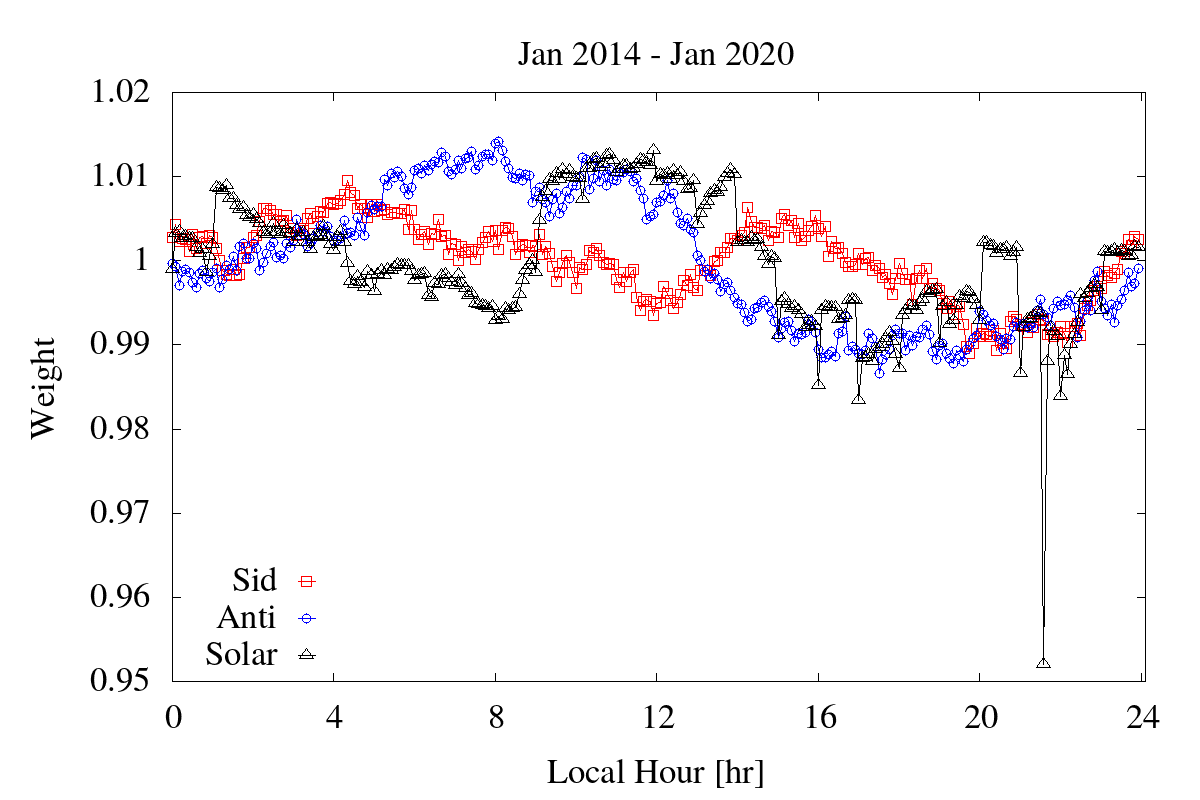
\includegraphics[width=0.5\textwidth]{weigth2014-2020_jan.png} 	
	\caption{Pesos de los hexágonos}
	\label{fig:wei_14_20}
\end{figure}

\section{Anisotropía}
El archivo de de todos los disparon empieza el Mon, 1 July 2013 12:05:08 GMT \footnote{$1372680308$}. Para trabajar en una cantidad entera de años, se trabaja a partir del  Thur, 1 January 2014 12:00:00 GMT \footnote{$1388577600$} y hasta el Thursday, 1 January 2020 12:00:00 GMT \footnote{$1577880000$}.  En este rango se tiene la tasa de eventos por día que se muestra en la Fig.\,\ref{tasa_total_diaria}.

% En el rango $1372680308$ \footnote{Mon, 1 July 2013 12:05:08 GMT} y $1388577600$ \footnote{Thur, 1 January 2014 12:00:00 GMT}, la tasa de eventos del archivo $\text{All Triggers}$, tenía una tasa de eventos por debajo de lo normal. Por esto, se utiliza los eventos a partir del  1388577600. La tasa de eventos que se utiliza se puede ver a continuación:

\begin{figure}[H]
	\centering
	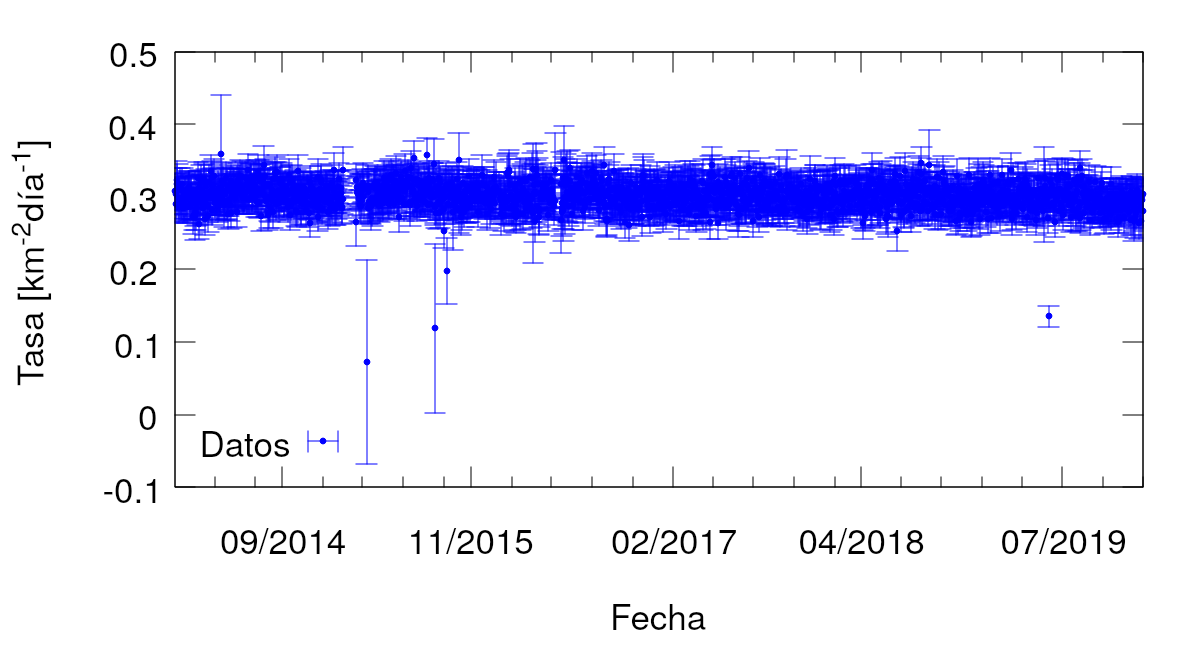
\includegraphics[width=0.5\textwidth]{rate_total.png}
	\caption{Tasa  de eventos en el rango de tiempo a trabajar}
	\label{tasa_total_diaria}
\end{figure}

\subsection{Lista detallada de los filtros aplicados de datos del herald}

\subsubsection{Datos para el análisis de anisotropía}
Esta sección muestra los filtros para los datos del análisis de anisotropía en el rango 1 EeV - 2 EeV.

\begin{enumerate}
	\item Energía entre  [1 EeV , 2 EeV)
	\item Rango de tiempo:
	\begin{itemize}
		\item[-] Inicial:1388577600 \\ (Thursday, 1 January 2014 12:00:00 GMT)
		\item[-] Final: 1577880000  \\ (Thursday, 1 January 2020 12:00:00 GMT)
	\end{itemize}
	\item Sectancia:  $\theta < 60^o$
	\item 6T5
	\item $ib=1$ Bad period flag. Un valor de 1 indica un buen periodo
\end{enumerate}

Con estos filtros se tienen $1\,092\,753$ eventos

\subsubsection{Datos para el cálculo de las correcciones del clima}

Estos son los filtros para los datos a utilizar para el cálculo de los parámetros del clima:

\begin{enumerate}
	\item Eventos con valor de señal de $S_{38}$\footnote{Valor de S38 sin la correccón del clima del paper del 2017} por encima de  $5.36\,\text{VEM}$. Este valor corresponde a $\sim 1\,$ EeV  en VEM.
	\item Rango de tiempo:
	\begin{itemize}
		\item[-] Inicial:1388577600 \\ (Thursday, 1 January 2014 12:00:00 GMT)
		\item[-] Final: 1577880000  \\ (Thursday, 1 January 2020 12:00:00 GMT)
	\end{itemize}
	\item Sectancia:  $\theta < 60^o$
	\item $iw<4$ (weather quality flag)
	\item 6T5
	\item $ib=1$ Bad period flag del herald.  Un valor de 1 indica un buen periodo
	\item $ib=1$ Bad period flag de los datos del clima. Un valor de 1 indica un buen periodo
\end{enumerate}


Con estos filtros se tienen $1\,208\,615$ eventos, con una tasa de eventos que se muestra en la Fig.\,\ref{tasa_total_diaria_ajuste_weather}. En la figura se observa que utilizando el corte en la señal de S38 sin corregir por la modulación del clima del herald \footnote{Las correcciones se calcularon para el archivo del disparo estándar} se observa una modulación anual.

\begin{figure}[H]
	\centering
	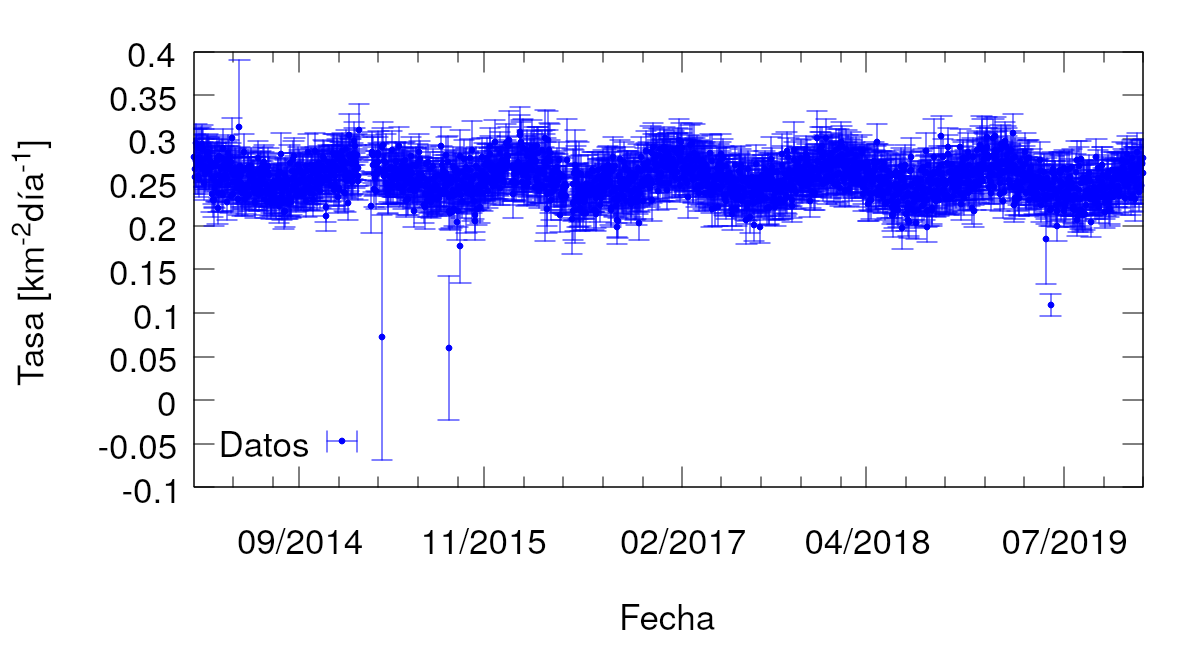
\includegraphics[width=0.5\textwidth]{rate_total_ajuste_weather.png}
	\caption{Tasa  de eventos en el rango de tiempo a trabajar para el ajuste de los parámetros del clima.}
	\label{tasa_total_diaria_ajuste_weather}
\end{figure}


\subsection{Análisis en frecuencia}

\begin{figure}[H]
	\centering
	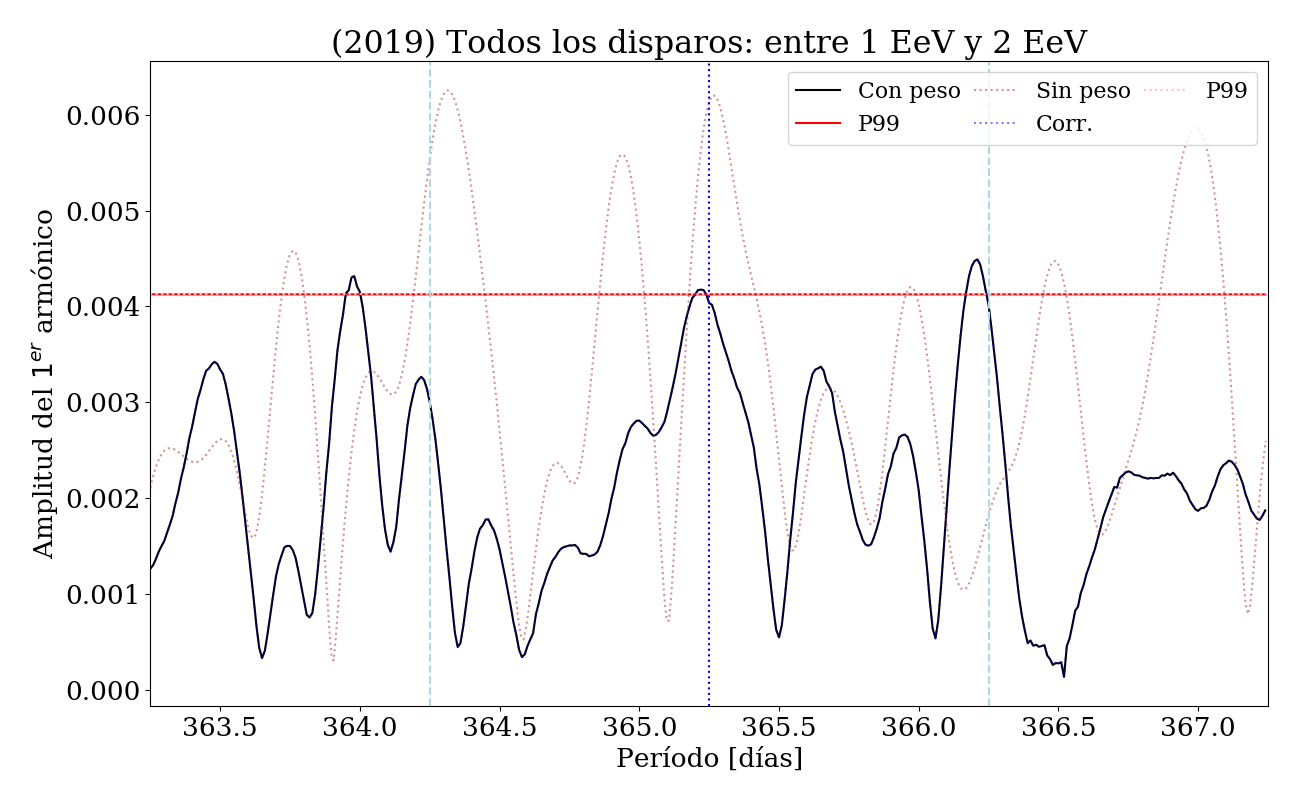
\includegraphics[width=0.5\textwidth]{2019_AllTriggers_1_2_EeV_con_vs_sin_peso.png}
	\caption{Análisis en frecuencia en ascensión recta en rango 1 EeV - 2 EeV}
	\label{fig:consin}
\end{figure}


\section{Corrección del clima}

\begin{figure}[H]
	\centering
	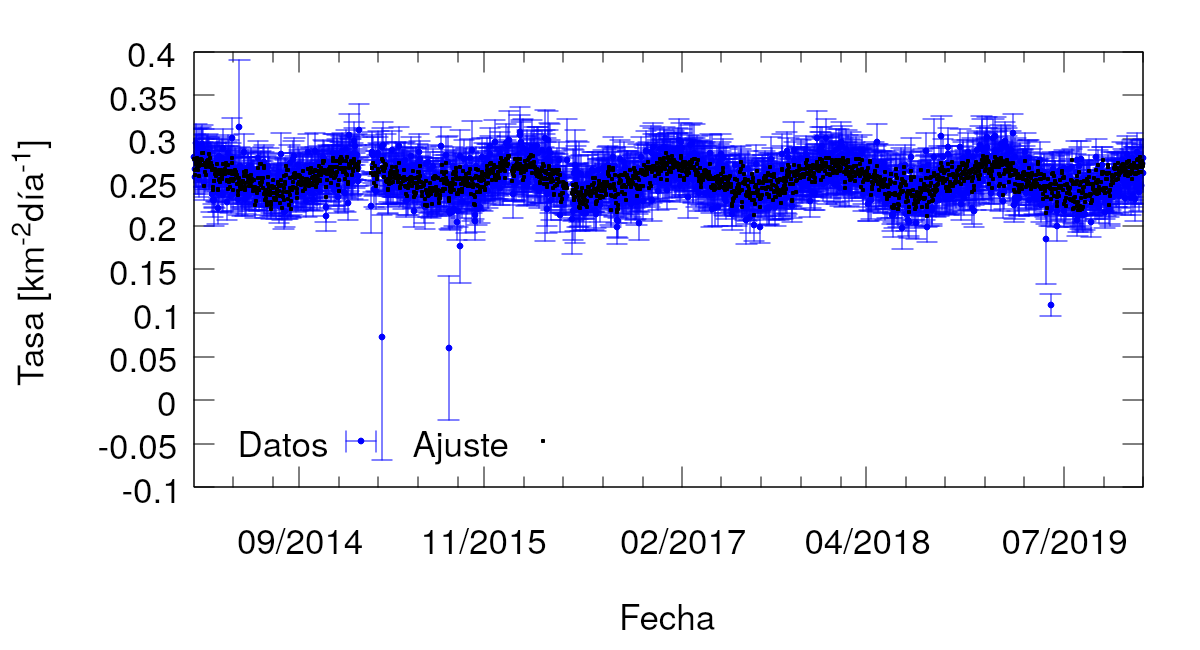
\includegraphics[width=0.5\textwidth]{rate_Ajuste.png}
\end{figure}



\begin{figure}[H]
	\centering
	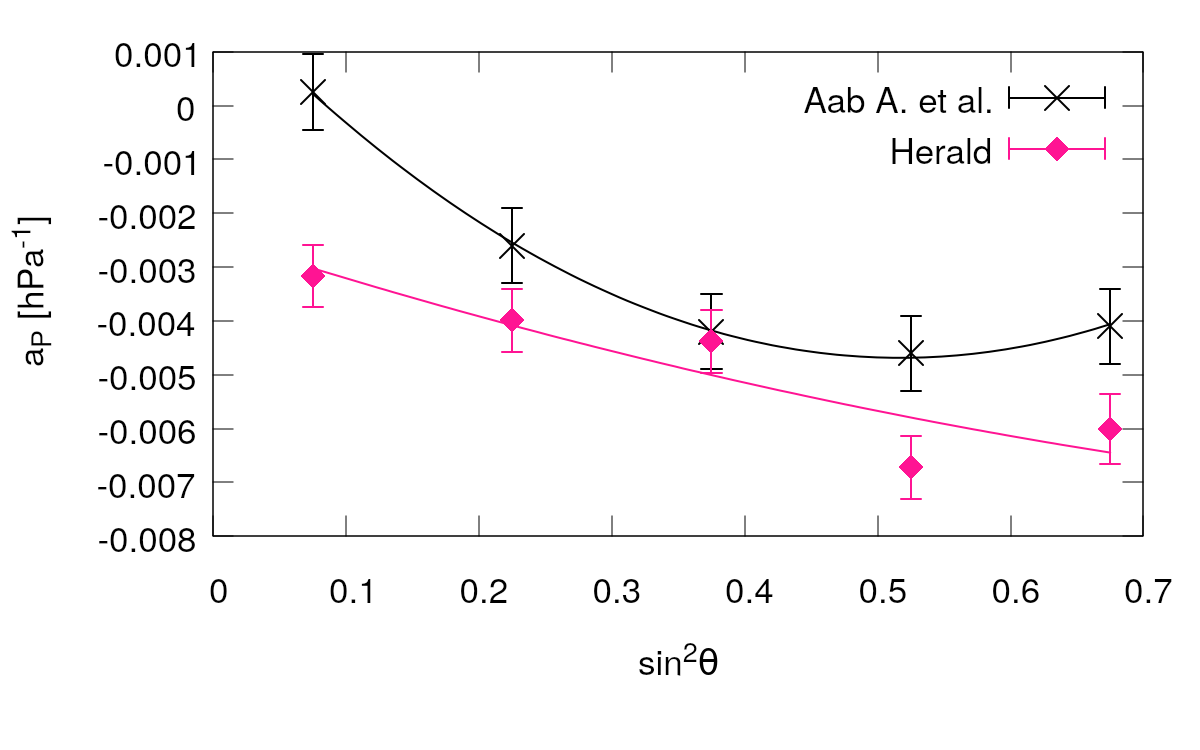
\includegraphics[width=0.5\textwidth]{ap_6t5.png}
	\caption{Parámetro de clima $a_P$ calculado para la corrección del archivo de todos los disparos}
\end{figure}

\begin{figure}[H]
	\centering
	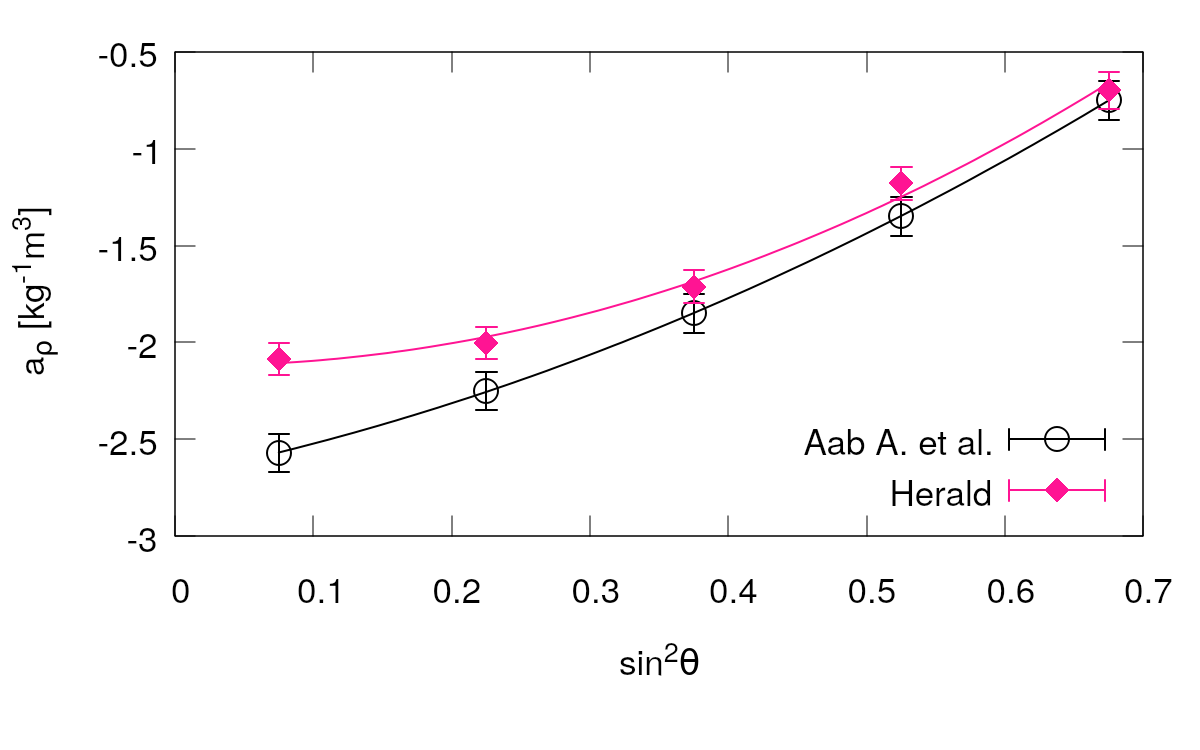
\includegraphics[width=0.5\textwidth]{arho_6t5.png}
	\caption{Parámetro de clima $a_\rho$ calculado para la corrección del archivo de todos los disparos}
\end{figure}

\begin{figure}[H]
	\centering
	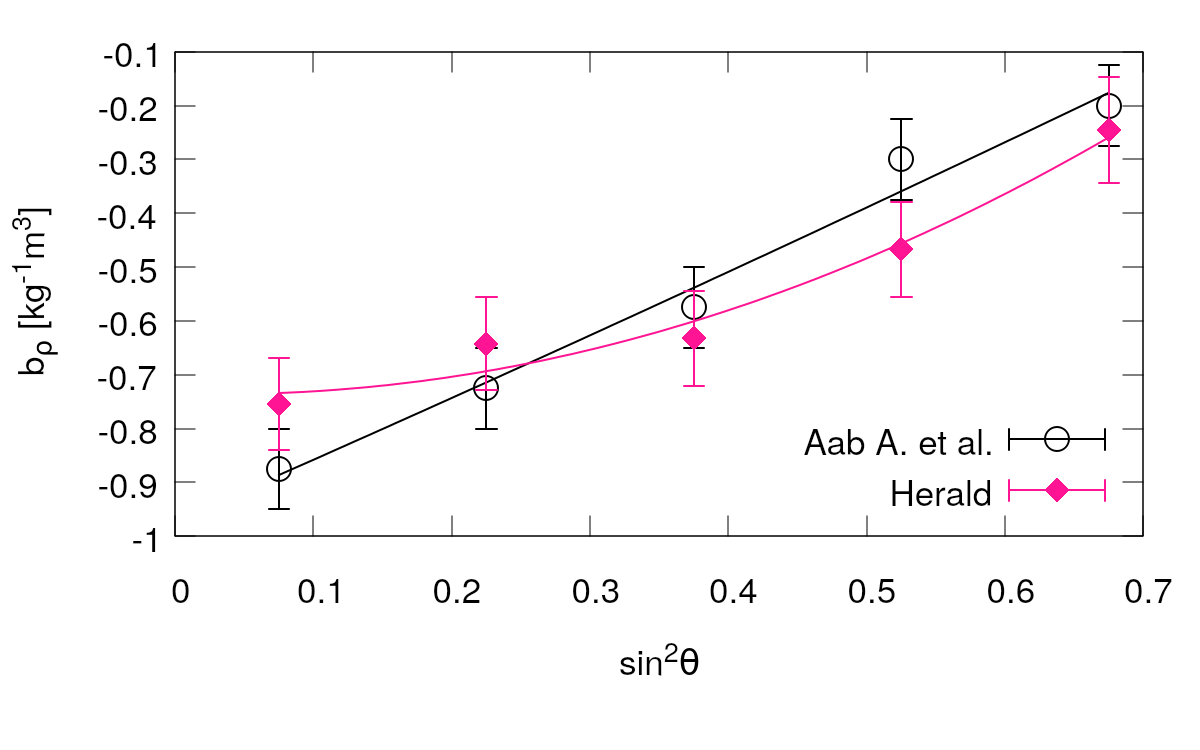
\includegraphics[width=0.5\textwidth]{brho_6t5.png}
	\caption{Parámetro de clima $b_\rho$ calculado para la corrección del archivo de todos los disparos}
\end{figure}

%%%%%%%%%%%%%%%%%%%%%%%%%%%%%%%%%%%%%%%%%%%%%%%%%%%%%%%%%%%%%%%%%%%%%%%%%%%%%%%%%%%%%%%%%
%%%%%%%%%%%%%%%%%%%%%%%%%%%%%%%%%%%%%%%%%%%%%%%%%%%%%%%%%%%%%%%%%%%%%%%%%%%%%%%%%%%%%%%%%
%%%%%%%%%%%%%%%%%%%%%%%%%%%%%%%%%%%%%%%%%%%%%%%%%%%%%%%%%%%%%%%%%%%%%%%%%%%%%%%%%%%%%%%%%

      \subsubsection{Modulación del clima para todos los triggers}

      Para corroborar los parámetros del clima, primero calculé las tasas de eventos de los archivos del 2017 y 2020 para energías mayores a 1  EeV, donde obtuve los siguientes gráficos Fig.\ref{fig:rate_daily_2017_1EeV} y \ref{fig:rate_daily_2020_1EeV}. 

        \begin{figure}[H]
        
          \begin{subfigure}[b]{0.5\textwidth}
          \centering
          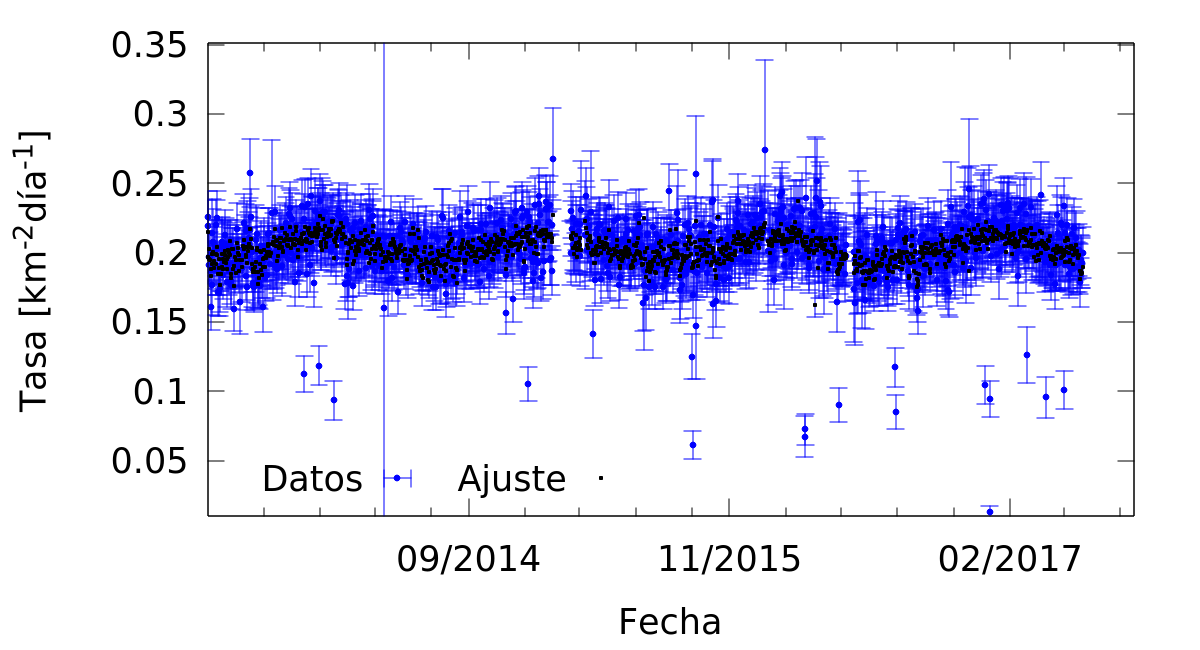
\includegraphics[width=\textwidth]{../0_Introduccion/daily_rate/daily_rate_AllTriggers_2017_1EeV.png}
          \caption{Archivo de 2017}   \label{fig:rate_daily_2017_1EeV}
          \end{subfigure}%
        \hfill
          \begin{subfigure}[b]{0.5\textwidth}
          \centering
          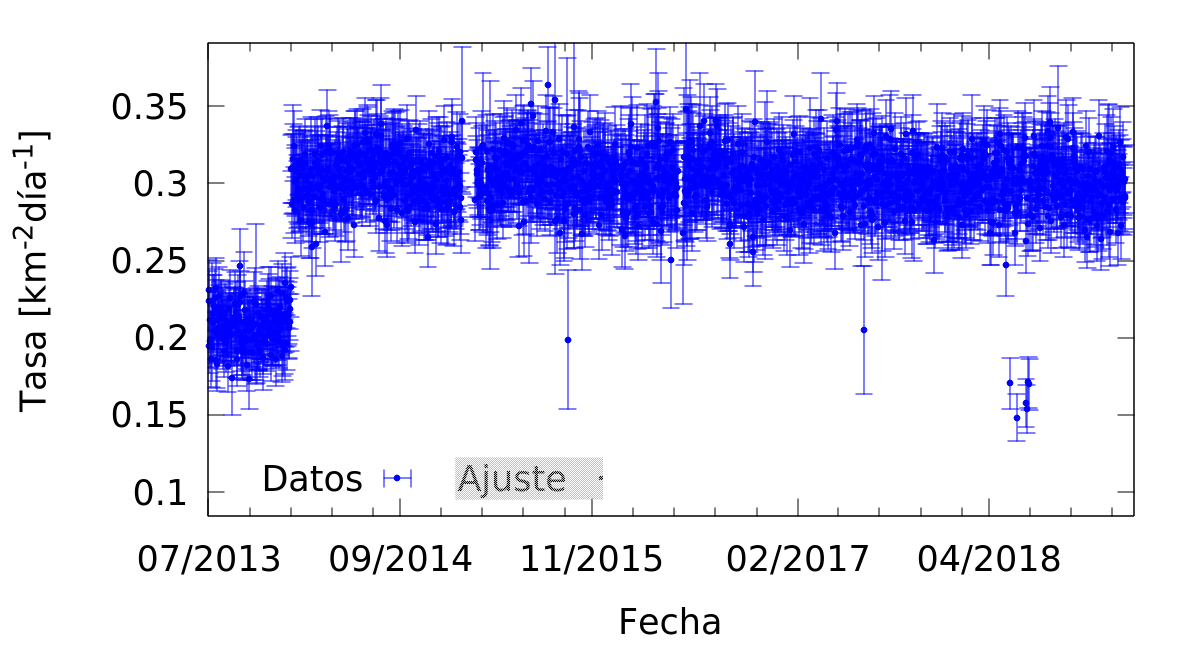
\includegraphics[width=\textwidth]{../0_Introduccion/daily_rate/daily_rate_AllTriggers_2019_1EeV.png}
          \caption{Archivo del 2020}  \label{fig:rate_daily_2020_1EeV}
          \end{subfigure}
          \caption{Tasa de eventos diaria por encima de 1 EeV para los datos de todos los disparos.}
        \end{figure}

      Después calculé los parámetros del clima para energía mayores a 1 EeV. Para el archivo de 2017 obtuve la Fig.\,\ref{fig:parameters_2017_1EeV}. Los comparé con el paper del weather del main array, para ver si dan algo razonable. Verifiqué las siguientes cosas para el ajuste

      \begin{itemize}
        \item Me fijé que delay en la densidad cada momento fuera de dos  horas
        \item Me fijé que el ajuste no tuviera en cuenta periodos malos, bad periods
        \item Me fijé que el delay de la densidad media también fuera tal que para cada evento estuviera centrada $\pm$12 horas
        \item También me fijé que el rango de tiempo estuviera bien, porque estos datos están disponibles desde el 2013  recién
        \item Me fijé que los $\chi^2$ reducido fuera algo razonable. Todos rondaban alrededor de $1.05$
      \end{itemize}

      EL rango de tiempo que usé fue este: 
      \begin{itemize}
        \item Inicio: 1372680308
        \item Final: 1496275090
      \end{itemize}
        \begin{figure}[H]
          \begin{subfigure}[b]{0.5\textwidth}
          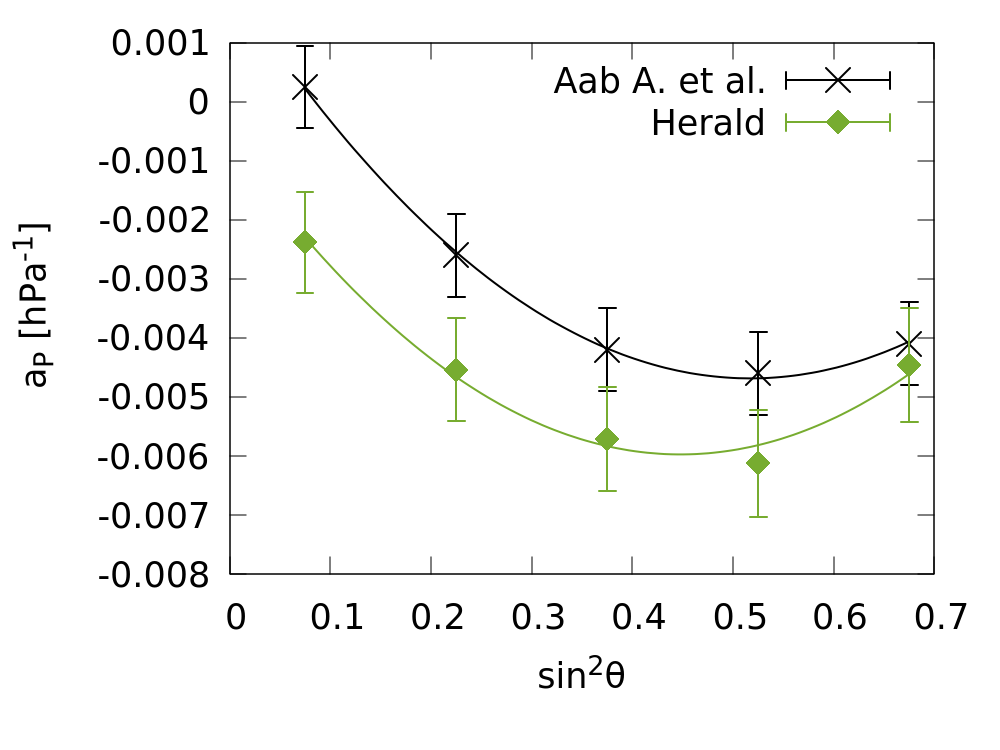
\includegraphics[width=\linewidth]{../0_Introduccion/params/ap_2017_above_1EeV.png}
          \caption{Parámetro $a_P$ }
          \label{fig:ap_2017_1EeV}
          \end{subfigure}%
          \hspace{\fill}
          \begin{subfigure}[b]{0.5\textwidth}
          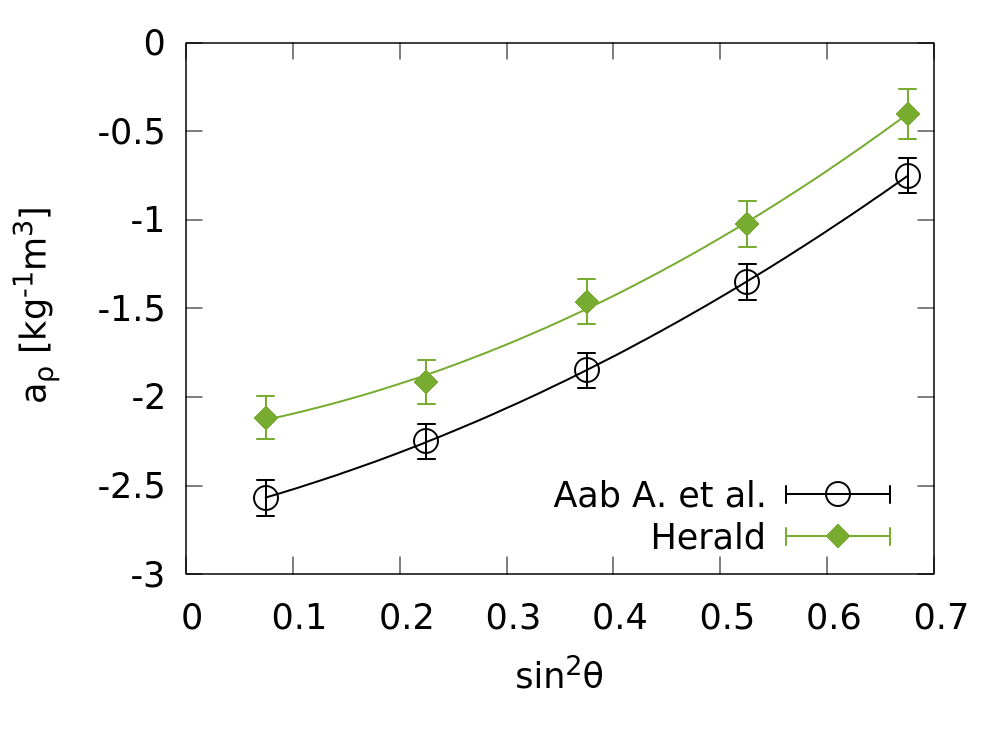
\includegraphics[width=\linewidth]{../0_Introduccion/params/arho_2017_above_1EeV.png}
          \caption{Parámetro $a_{\rho}$ }
          \label{fig:arho_2017_1EeV}
          \end{subfigure}%
          \hspace{\fill}
          \begin{subfigure}[b]{\textwidth}
          \centering
          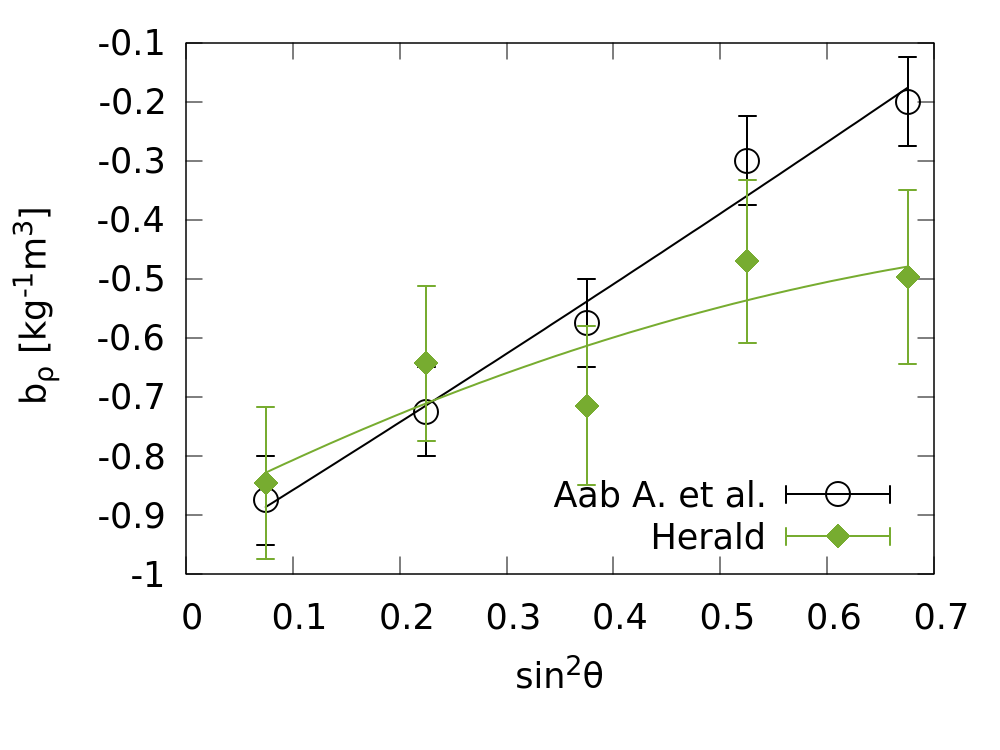
\includegraphics[width=0.5\linewidth]{../0_Introduccion/params/brho_2017_above_1EeV.png}
          \caption{Parámetro  $b_\rho$   }
          \label{fig:brho_2017_1EeV}
          \end{subfigure}%
          \caption{Parámetros de la modulación del clima considerando los datos para todos los disparos de 2017. Los mismos se comparan con los ajustes obtenidos en \cite{aab2017impact}.}\label{fig:parameters_2017_1EeV}
        \end{figure}

        Lo que más me llama la atención es el comportamiento del parámetro $b_\rho$, que como se discutió en otras oportunidades, tiene que ver con el parámetro $a_\rho$ con una razón de  $1:3$ más o menos. 



      Hacemos el mismo procedimiento con el archivo 2020, {\bf pero filtrando los eventos por el valor de S38 sin corregir por la modulación del clima}. Para calcular la tasa y los parámetros del clima, se toman los eventos después de ese salto de 0.2 a 0.3, obtengo los siguientes resultados:

        \begin{figure}[H]
          \centering
          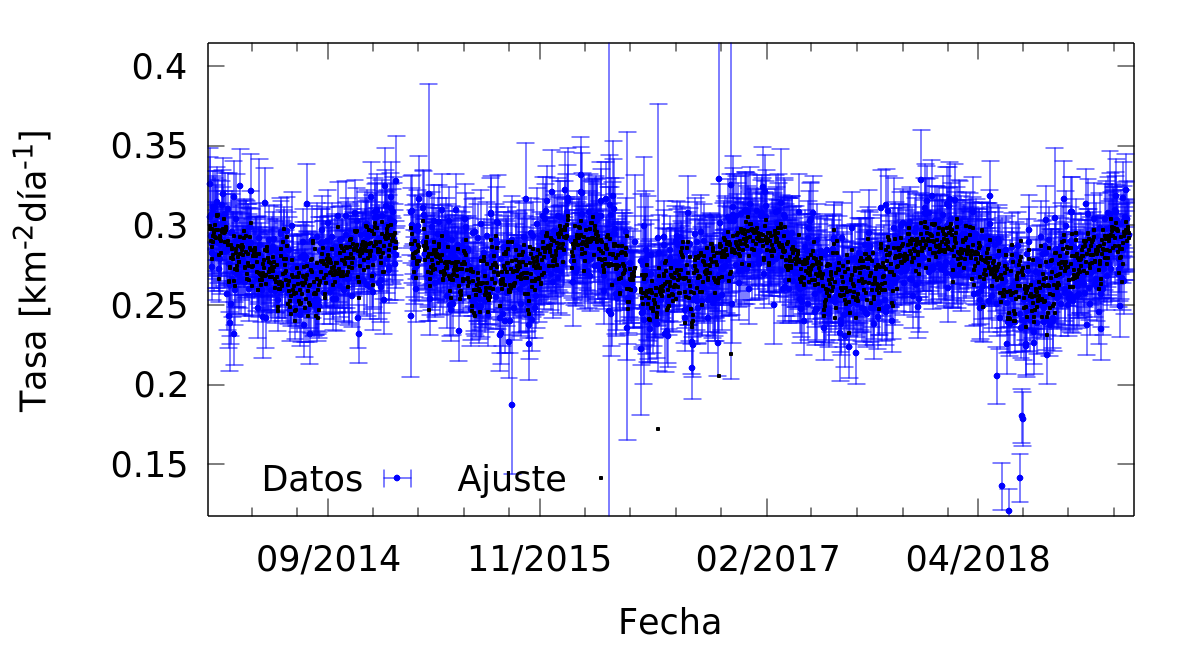
\includegraphics[width=0.5\textwidth]{../0_Introduccion/daily_rate/daily_rate_AllTriggers_2020_1EeV.png}
        \end{figure}

      Acá también verifiqué lo mismo que el caso anterior, lo único que ahora el $\chi^2$ rondaba alrededor de los $1.08$. Siempre verifico que no sea mucho mayor o menor a 1.

      EL rango de tiempo que usé para este caso fue este: 
      \begin{itemize}
        \item Inicio: 1388910508
        \item Final: 1550490858
      \end{itemize}
      
        \begin{figure}[H]
          \begin{subfigure}[b]{0.5\textwidth}
          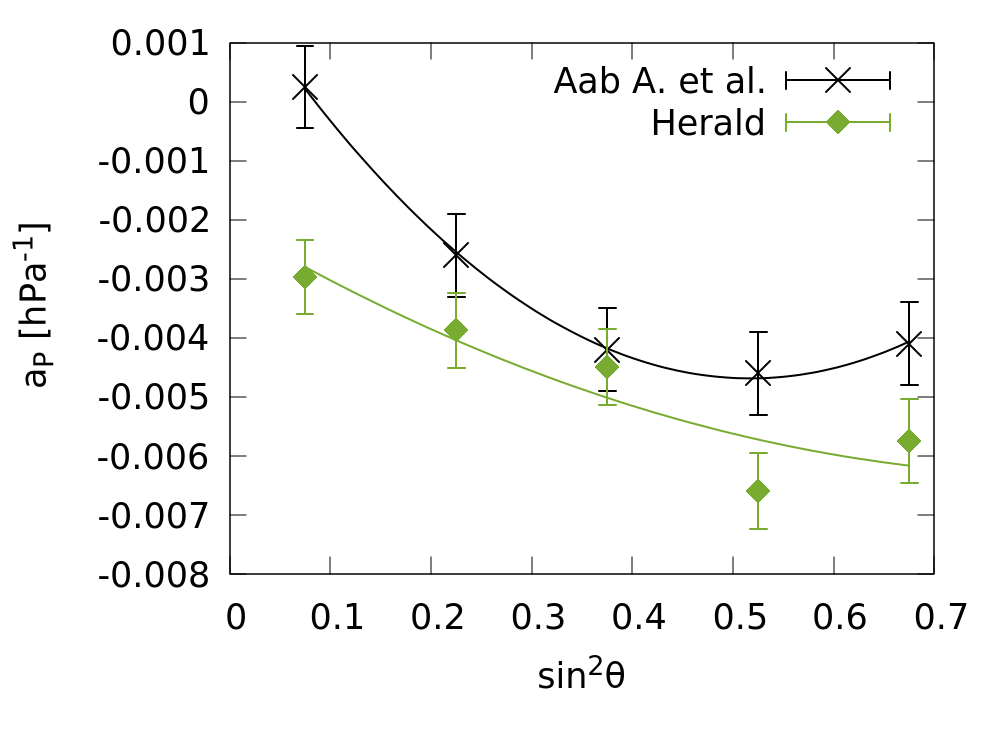
\includegraphics[width=\linewidth]{../0_Introduccion/params/ap_2020_above_1EeV.png}
          \caption{Parámetro $a_P$ }
          \label{fig:ap_2020_1EeV}
          \end{subfigure}%
          \hspace{\fill}
          \begin{subfigure}[b]{0.5\textwidth}
          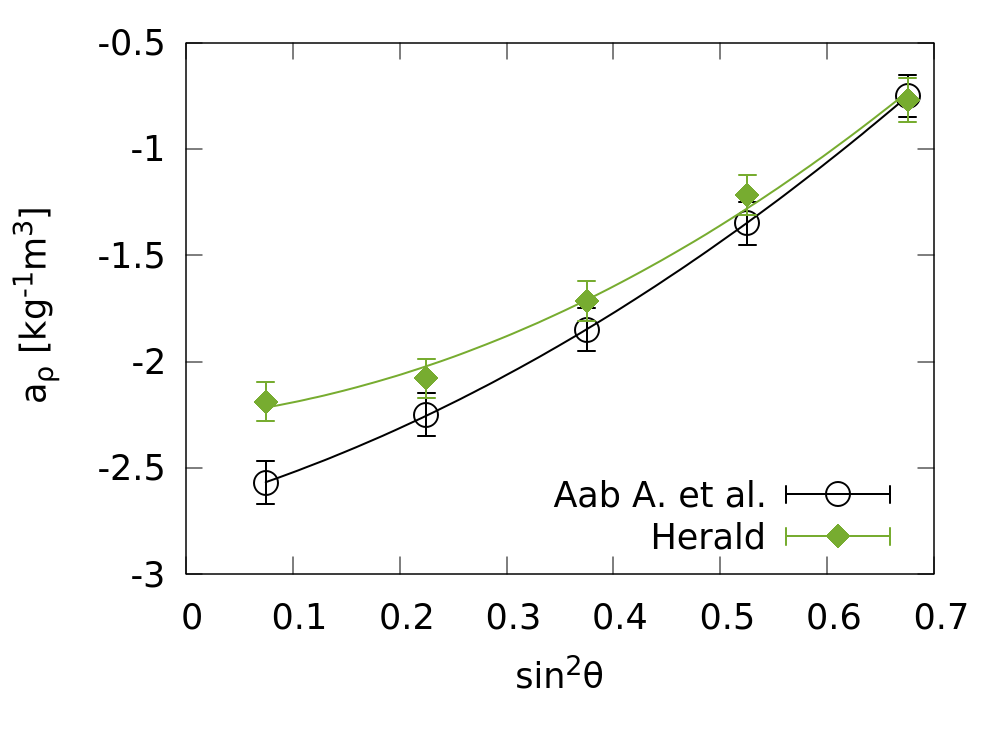
\includegraphics[width=\linewidth]{../0_Introduccion/params/arho_2020_above_1EeV.png}
          \caption{Parámetro $a_{\rho}$ }
          \label{fig:arho_2020_1EeV}
          \end{subfigure}%
          \hspace{\fill}
          \begin{subfigure}[b]{\textwidth}
          \centering
          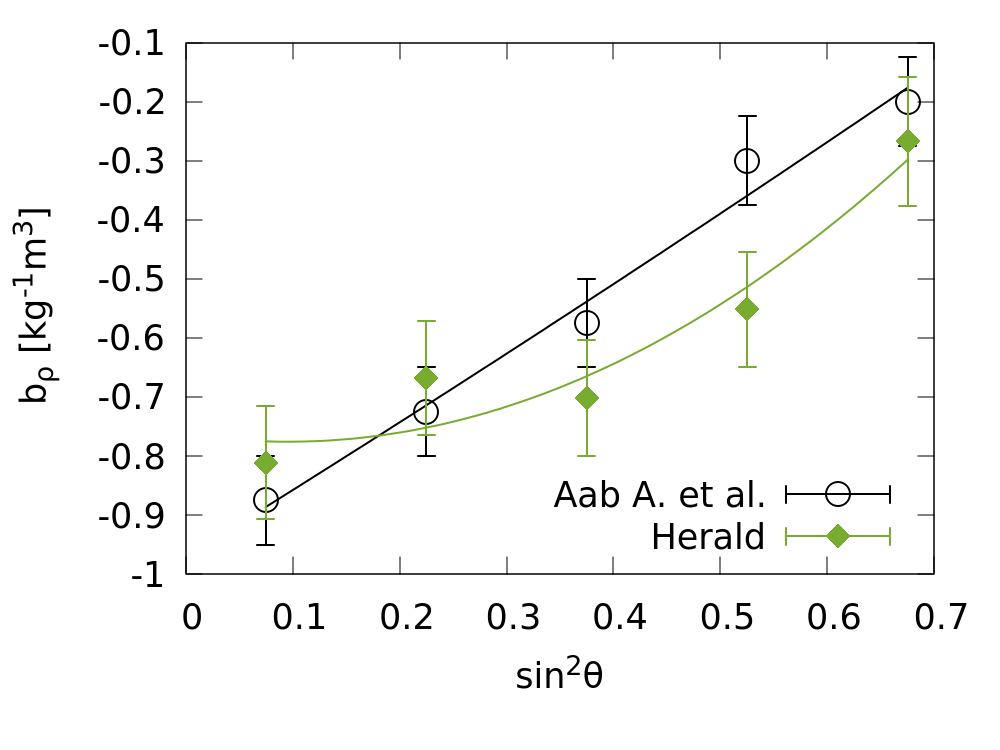
\includegraphics[width=0.5\linewidth]{../0_Introduccion/params/brho_2020_above_1EeV.png}
          \caption{Parámetro  $b_\rho$   }
          \label{fig:brho_2020_1EeV}
          \end{subfigure}%
          \caption{Parámetros de la modulación del clima considerando los datos para todos los disparos de 2020. Los mismos se comparan con los ajustes obtenidos en \cite{aab2017impact}.}\label{fig:parameters_2020_1EeV}
        \end{figure}



      Considerando el filtro con el S38 en el archivo 2020 y la energía en el 2017, quiero saber si obtengo parametros  del clima comparables. Ya que el Main Array se corresponden los parametros del 2015 y 2019, yo esperaría que con todos los triggers pase los mismo. Una diferencia importante entre ambos análisis es que los parametros del 2020 contienen eventos hasta el 31/12/2019.


        \begin{figure}[H]
          \begin{subfigure}[b]{0.5\textwidth}
          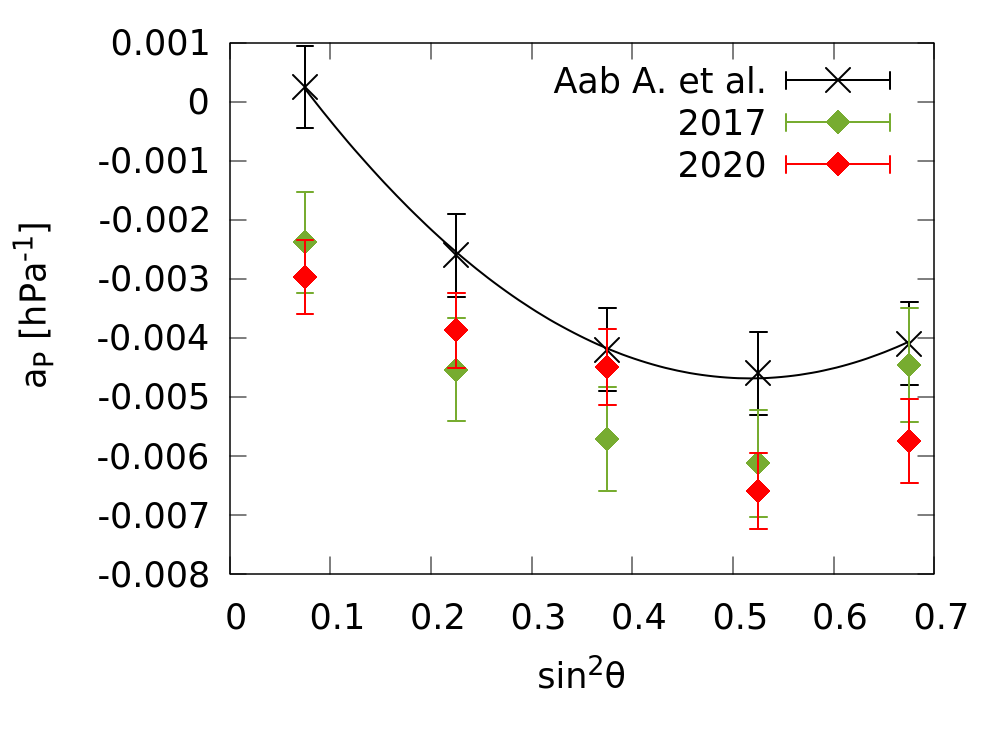
\includegraphics[width=\linewidth]{../0_Introduccion/params/ap_2017_2020_above_1EeV.png}
          \caption{Parámetro $a_P$ }
          \end{subfigure}%
          \hspace{\fill}
          \begin{subfigure}[b]{0.5\textwidth}
          \includegraphics[width=\linewidth]{../0_Introduccion/params/arho_2017_2020_above_1EeV.png}
          \caption{Parámetro $a_{\rho}$ }
          \end{subfigure}%
          \hspace{\fill}
          \begin{subfigure}[b]{\textwidth}
          \centering
          \includegraphics[width=0.5\linewidth]{../0_Introduccion/params/brho_2017_2020_above_1EeV.png}
          \caption{Parámetro  $b_\rho$   }
          \end{subfigure}%
          \caption{Parámetros de la modulación del clima considerando los datos para todos los disparos del archivo 2017 y 2020. Los mismos se comparan con los ajustes obtenidos en \cite{aab2017impact}.}
        \end{figure}

      Se ve que estos parametros no son comparables. 


\chapter{Report \#5: 22/05/2020 - Dipolo en el bin 1 EeV - 2 EeV}
\graphicspath{{report_5_22_05_2020/}}
\section{Anisotropías}

\subsubsection{Características del conjunto de datos del reporte}

\begin{itemize}
	\item Energía entre  [1 EeV , 2 EeV)
	\item Rango de tiempo:
	\begin{itemize}
		\item[-] Inicial:1388577600 (Thursday, 1 January 2014 12:00:00 GMT)
		\item[-] Final: 1577880000  (Thursday, 1 January 2020 12:00:00 GMT)
	\end{itemize}
	\item Sectancia:  $\theta < 60^o$
	\item 6T5
	\item $ib=1$ Bad period flag. Un valor de 1 indica un buen periodo
	\item Número de eventos: $1\,081\,844$
\end{itemize}


\begin{figure}[H]
	\centering
	\includegraphics[width=0.8\linewidth]{../report_4_12_05_2020/2019_AllTriggers_1_2_EeV_con_vs_sin_peso.png}
	\caption{Anisotropía para el intervalo 2014-2020}
	\label{fig:anis}
\end{figure}

\begin{table}[H]
\centering
\begin{tabular}{l|c|c}
				& Con Peso 	& Sin peso 		\\ \hline
Frecuencia:		& 366.25 	& 366.25 		\\
Fase:			& 329.865 	& 292.312		\\
$P(r)$:			& 0.76398\%	& 26.6838 \% 	\\
Amplitud:		& 0.004676 	& 0.00243515	\\
\end{tabular}
\caption{Fase, $r_{99}$ y $P_{99}$ del análisis de anisotropía entre en 1 de Enero del 2014 y el 1 de Enero del 2020}
\end{table}



En la Fig.\ref{fig:zoom} se muestra el pico que se presenta en  el intervalo de energía entre 1 EeV - 2 EeV, cercano a la frecuencia sidérea. El pico tiene un máximo para un período de $366.21$. En la Tabla.\,\ref{tabla:pico} se muestran los valores de la fase, $r_{99}$ y $P_{99}$ para el periodo anterior.

\begin{figure}[H]
	\centering
	\includegraphics[width=0.5\linewidth]{zoom_anis.png}
	\caption{Zoom en el pico de anisotropía cercana para la frecuencia sidérea para el intervalo 2014-2020}
	\label{fig:zoom}
\end{figure}



\begin{table}[H]
\centering
\begin{tabular}{l|c|c|c|c}
				& Con Peso 		& Sin peso 		& Con Peso 		& Sin peso 		\\ \hline
Frecuencia:		& 366.21 		& 366.21 		& $\sim$366.505 & 366.506 		\\
Fase:			& 151.032 		& 121.695		& $\sim$190 	& 73.8188		\\
$P(r)$:		& 0.289882\%	& 46.9691 \% 	& $\sim$96\%	& 0.24013 \% 	\\
Amplitud:		& 0.00512146	& 0.0018417		& $\sim$0.0006	& 0.00520328	\\
\end{tabular}
\caption{Fase, $r_{99}$ y $P_{99}$ del análisis de anisotropía entre en 1 de Enero del 2014 y el 1 de Enero del 2020}
\label{tabla:pico}
\end{table}


\section{Ajuste del primer armónico de la variación de hexágonos y pesos}

Para verificar los valores de amplitud y fase en la frecuencia sidérea, se ajusta una función del tipo 
\begin{equation}
	f(RA) = a\cos{(2\pi(\omega RA + \phi))} +c
\end{equation}

a la variación de los hexágonos por ángulos de ascensión recta $RA$, así como también a la variación de los pesos de los eventos en ascensión recta \footnote{El peso de los eventos es la inversa del peso de los hexágonos}. En el ajuste, se dejan libres los parámetros de la amplitud $a$, desfase $\phi$ y offset $c$, en cambio la frecuencia $\omega=1$, ya que los valores de ascensión recta $0^o$ y $360^o$ son equivalentes y estamos trabajando con el primer armónico. La variación y el ajuste puede verse en las Figs.\ref{fig:pesos_ajuste} y \ref{fig:pesos_hexagonos}.

\begin{figure}[H]
	\centering
	\includegraphics[width=0.5\linewidth]{ajuste_pesos.png}
	\caption{Pesos de los eventos en función de la ascensión recta para la frecuencia sidérea en el periodo 2014-2020}
	\label{fig:pesos_ajuste}
\end{figure}


\begin{figure}[H]
	\centering
	\includegraphics[width=0.5\linewidth]{ajuste_hexagonos.png}
	\caption{Hexágonos para la frecuencia sidérea en el periodo 2014-2020}
	\label{fig:pesos_hexagonos}
\end{figure}


Los valores de los ajustes, comparados con el análisis de Rayleigh se muestran en la Tabla\,\ref{tabla:ajuste_primer_armonico}. SE observa que el valor de la amplitud para el caso de la variación de los pesos es más cercana al que se obtuvo en el análisis de Rayleigh. Esto puede deberse que los pesos están normalizados por la integral de todos los hexágonos dada un frecuencia, por lo que si existe alguna constante multiplicativa en la cantidad de hexágonos, la amplitud la tabla para la primera columna puede no ser igual a la segunda columna.

\begin{table}[H]
\centering
\begin{tabular}{l|c|c|||c}
				& Hexágonos 				& Pesos	de los eventos		& Rayleigh con peso \\ \hline
Figura:			& \ref{fig:pesos_hexagonos} &\ref{fig:pesos_ajuste}		&\ref{fig:zoom} \\
Fase $\phi$:	& 284.874 	 				& 285.099					&329.865	\\
Amplitud $a$:	& 0.00784107 				&  0.00384774 				&0.004676\\
\end{tabular}
\caption{Fase y amplitud del ajuste del primer armónico en ascensión recta en los hexágonos y  pesos  de los eventos para la frecuencia sidérea}
\label{tabla:ajuste_primer_armonico}
\end{table}


\chapter{Dipolo en el bin 1 EeV - 2 EeV}
\graphicspath{{report_6_02_06_2020/}}
	\section{Características del conjunto de datos} \label{specs}
	

	Además de los filtros aplicados mencionados en la sección \ref{filtro}, se aplican filtros adicionales sobre la energía y el rango de tiempo. Para estudiar los eventos en esta sección, consideramos los eventos entre 1\,EeV y 2\,EeV de energía y que ocurrieron entre las $12:00:00$ GMT del 1 de enero de 2004 y las $12:00:00$ GMT del 1 de enero de 2020. Se  eligió ese rango de tiempo, ya que el registro de eventos más reciente al que se tuvo para hacer este trabajo termina el 1 de Enero del 2020   a las $11:59:43$ GMT, además de para estudiar una cantidad entera de años, se optó por considerar los eventos desde el 1 de Enero del 2013 a las $12:00:00 $ GMT.

	Un resumen de todos los filtros aplicados se encuentra a continuación
		\begin{enumerate}
			\item Son eventos obtenidos mediante todos los disparos.
			\item Energía entre  [1 EeV , 2 EeV)
			\item Rango de tiempo:
			\begin{itemize}
				\item[-] Inicial:1388577600 (Jueves, 1 de Enero de 2014 12:00:00 GMT)
				\item[-] Final: 1577880000  (Jueves, 1 de Enero de 2020 12:00:00 GMT)
			\end{itemize}
			\item Ángulo cenital $\theta < 60^o$
			\item 6T5
			\item $ib=1$ Bad period flag. Un valor de 1 indica un buen periodo
		\end{enumerate}
	Aplicando estos filtros, se tienen $1\,081\,844$ eventos para estudiar en este rango de energía.


\section{Pesos de los eventos para frecuencias de referencia}

Se toman las frecuencia anti-sidérea ($f_a=364.25\,$ciclos), solar ($f_{Solar}= 365.25\,$ciclos) y sidérea ($f_{sid}= 366.25\,$ciclos) como referencia para obtener una aproximación a primer orden del análisis en frecuencias. A cada una de estas frecuencias, se ajusta una función del tipo  $f(x)=a\cdot \cos{(\alpha-\phi)} + 1$, con el se busca aproximar la amplitud $a$ y el desfase $\phi$ de las curvas de los pesos en función de la ascensión recta $\alpha$. Los ajustes se observan en las Figs. \ref{fig:ajuste_antisiderea}, \ref{fig:ajuste_solar} y \ref{fig:ajuste_siderea}.


\subsection{Gráficos de los ajustes}


\begin{figure}[H]
\begin{subfigure}{.5\textwidth}
	\centering
	\includegraphics[width=\linewidth]{eventos_RA_ajuste_cos_antisiderea_v2.png}
	\caption{Frecuencia anti-sidérea}
	\label{fig:ajuste_antisiderea}
\end{subfigure}%
\begin{subfigure}{.5\textwidth}
	\centering
	\includegraphics[width=\linewidth]{eventos_RA_ajuste_cos_solar_v3.png}
	\caption{Frecuencia solar}
	\label{fig:ajuste_solar}
\end{subfigure}\\
\centering
\begin{subfigure}{.5\textwidth}
	\centering
	\includegraphics[width=\linewidth]{eventos_RA_ajuste_cos_siderea_v2.png}
	\caption{Frecuencia sidérea}
	\label{fig:ajuste_siderea}
\end{subfigure}%
\caption{Ajuste de los pesos de los eventos para varias frecuencias a primer orden en ascensión recta}
\end{figure}

	
\subsection{Tabla comparando los ajustes:}
		
		\begin{table}[H]
		\centering
		\begin{tabular}{c|c|c|c}
					& Anti-sidérea			& Solar 				& Sidérea\\ \hline
		Fase $\phi$ & $0.0109\pm 0.0003 $ 	&	$0.0038 \pm 0.0003$	&  $0.0047\pm 0.0007$		\\
		Amplitud $a$& $15    \pm 1$ 		&   $360 \pm 5   $ 		&  $31    \pm 8    $ 		\\
		\end{tabular}
		\caption{Parámetros obtenidos del ajuste a primer orden en $\alpha$ sobre los pesos.}
		\end{table}


\section{Gráfico de la anisotropía}
		
	\subsubsection{Análisis de anisotropías en ascensión recta}
		
		\begin{figure}[H]
			\centering
			\includegraphics[width=\linewidth]{pesos_sin_con_1_2_EeV.png}
			\caption{Anisotropía en función de la frecuencia, se comparan los análisis sin los pesos y con los pesos de los hexágonos}
		\end{figure}
		
		
		\begin{table}[H]
		\centering
		\begin{tabular}{c|c|c|c|c|c}
					& Solar (sin peso)	& Solar (con peso)	&& Sidérea (sin peso) 	& Sidérea (con peso)	 \\ \hline
		Fase $\phi$ & 251	    		& 288	    		&& 289				& 335				\\
		Amplitud $r$& 0.0061	    	& 0.0038	  		&& 0.0041			& 0.0039			\\
		\end{tabular}
		\caption{Comparación de los parámetros de fase y amplitud para las frecuencias sidérea y solar, analizando sin pesos y con los pesos de los hexágonos con el análisis de Rayleigh}
		\end{table}


\subsubsection{Bineado de eventos }


Considerando que estamos trabajando con la frecuencia solar al hacer el análisis con pesos, se obtiene la siguiente distribución de eventos en función de su ascensión recta.
\begin{figure}[H]
	\centering
	\includegraphics[width=\linewidth]{eventos_clasificados_por_RA_v2.png}
	\caption{Distribución de la cantidad relativa de eventos en función de la ascensión recta.}
\end{figure}

% Si realizamos un ajuste de una función del tipo $f(x) = a\cdot\cos{(x - \phi)}) + 1 $, se obtiene los siguientes valores
		
% 	Fase $\phi$ : $288(60)^o$  \\
% 	Amplitud $a$: 0.002(2)  	\\





\appendix
\chapter{Cosas para hacer:  Mails con Mollerach}
% Fecha: 13/05/2020

% \begin{itemize}
% 	\done Para calcular los coeficientes del weather, queremos los mejores eventos, asi que tambien se usan solo los 6T5 (no es tan importante ganar un poquito mas de estadistica arribade 4 EeV para eso).

% 	\done En resumen usa los cortes 6T5 y $\theta<60$ para anisotropias y para weather correction.

% 	\done El corte de quality weather flag solo se usa para seleccionar los eventos para calcular las correcciones del weather.

% 	\done Los resultados nuevos son un poco raros, en siderea desaparecio toda la señal cuando pones pesos 1, y despues crece algo con los pesos. Revisa con los cortes bien puestos.

% 	\done Pone una tabla con amplitud y fase con y sin peso tambien.
% \end{itemize}


% Fecha: 20/05/2020

% \begin{itemize}

% 	\done Una cosa que se me ocurre es que al plot de hexagonos en frecuencia siderea le fitees un coseno. De ahi saca la amplitud del primer armónico de la modulación y la fase en RA donde esta el maximo.

% 	\done Despues hace el analisis de anisotropia en los eventos sin pesos y con pesos, y obtene la amplitud de la modulación y las fases del máximo en ambos casos.

% 	\done De ahi podriamos ver comparando las cantidades vectoriales (no solo la amplitud de la modulacion sino para donde apunta) qué es lo que esta pasando.

% 	\done Haceme un mail con esos resultados cuando los tengas, a ver si entendemos eso.
% \end{itemize}


Fecha: 27/05/2020

% \begin{itemize}
% 	\done los eventos son los 6T5 con cenit < 60 grados? Cuantos eventos son? (Pone siempre esos datos asi se sabe de quienes hablas)
% 	\done En la parte que fiteas el coseno, estas dejando libre una frecuencia, w en tu formula? 
% 	\done Lo que es relevante en el analisis que hacemos es el primer armonico de la funcion, aunque no de un buen fit. lo que afecta el valor del dipolo va ser la amplitud y fase en 1+A*cos(RA-B). Proba hacer ese fit y reporta los valores de A y B
% 	\done Otra cosa, no entiendo porque la figura de hexagonos y la de pesos tienen el maximo y minimo en los mismos valores. Los pesos son proporcionales a la inversa de los hexagonos.
% 	\done Porque no es periodica
% \end{itemize}


% Fecha: 28/05/2020

% \begin{itemize}
	% \done llama la atencion la modulacion de los hexagonos y de los pesos que pones en la tabla 1.3. Deberian tener aprox la misma amplitud y fase opuesta. Creo que estan mal los valores del fit a los hexagonos, deberia ser a ojo una amplitud cerca a 0.0035 y una fase cerca de 100. Igual es raro porque las curvas en el plot tienen pinta razonable. Fijate que cuando fiteas un coseno 1+A*cos(RA-B) va con menos B, asi B es la fase donde la funcion tiene el maximo. Fijate que si fiteas a una funcion con media distinta de 1, la amplitud es el factor A en C*(1+A*cos(RA-B)) y  no el factor  A en C+A*cos(RA-B)

	% \item 
	el test que queriamos hacer para ver si son compatibles las amplitudes de Fourier del primer armonico con y sin peso con la modulacion de los pesos no estaria funcionando. La idea es que si sumas vectorialmente un vector con amplitud igual a amplitud del primer armonico sin pesos apuntando en la direccion de la fase sin pesos mas otro vector con amplitud igual a la del fit a los pesos de los eventos apuntando en la fase del maximo del coseno, el vector suma deberia tener amplitud igual a la amplitud del analisis de fourier con pesos y apuntar en la direccion de la fase de ese analisis. No se en cual de los pedazos estara el error.
	
	% \item Para ir chequeando todo podrias:

	% \begin{itemize}
	
	% 	\done  binear los eventos en RA, por ejemplo en bines de 10 grados. 
		
	% 	\done Plotear el numero de evento en cada bin dividido la media (esta va a ser Ntotal/36) en funcion de la RA. 
		
	% 	\done Fitearle un coseno 1+A*cos(RA-B) a ese plot, te deberia dar aprox lo mismo que hacer el analisis de Fourier de los eventos sin peso. Asi podes comprobar si ese analisis te esta dando bien. Ademas es lindo hacer el plot y mostrar la distribucion en RA de los eventos.

	% 	\done  despues haces lo mismo poniendole los pesos a los eventos y comprobas si estas haciendo bien el analisis de Fourier con pesos.
	
	% 	\done  Me acabo de acordar que en algun momento tenias un lio con el  cero de donde contar la ascencion recta. Asegurate que los pesos los estas poniendo con la fase correcta, o sea que el tiempo sidereo en el que pones los hexagonos se corresponde bien con la RA del cenit del observatorio en ese momento (me parece que el problema podria venir de un corrimiento del cero, ya que eso da un error en la fase de los hexagonos)
	% \end{itemize}
%\end{itemize}


% Fecha: 09/06/2020

% Hay algunas cosas, al menos de notación, que  seria bueno mejorar y ver que no esten afectando los resultados.

% \begin{itemize}
	% \item
	% \done No cambies la notación de los papers de Auger( y la tesis de Oscar) para evitar confusiones. En particular, siguiendo la numeracion de tus puntos:

	% \begin{itemize}
	% 	\done 1 - periodo T: aca pones el periodo en segundos de la frecuencia que queres estudiar? por ejemplo para solar 24x3600? y para siderea 24x3600*365.25/366.25?

	% 	\done 2 - hora local se entiende la hora del reloj en Malargue. Mejor usa t en vez de hora local, aclarando que es el utc del evento (no tiene que estar entre 0 y 24 hs)

	% 	\done - Parece que estas intercambiando lo que normalmente se entiende como frecuencia y lo que se entiende como periodo:
	% 	\item

	% 		\begin{itemize}

	% 			\done la frecuencia solar equivale a $\sim$ 365,25 ciclos por año, y el periodo es la duracion de cada ciclo, y siempre se denoto con T, asi que seria mas correcto definir la coordenada angular asociada a cada frecuencia f\_x (sol, sid, antisid,..., con periodo T\_x), medida por ejemplo en horas,  como 

	% 			$h_x= 24 \frac{t-t_0}{T_x} + h_x(t_0)$

	% 			(en tu ecuacion parece estar al reves, o sea $T_x$ multiplicando, fijate si esta bien en el programa)

	% 			\done  para el grafico de las amplitudes para distintas frecuencias no importa el valor de $h_x(t_0)$, solo que tiene que ser consistente el valor para los hexagonos y los eventos, asi que ahi eventualmente podes tomar simplemente$ h_x=24  t/T_x$  (si queres el resultado en horas, yo te aconsejaria ponerlo directamente en radianes para el analisis de Fourier, reemplazando 24 por 2 pi)

	% 			\done Si queres calcular la fase siderea, sí es importante que h\_sid coincida con el right ascension, y sabemos que el right ascension del zenith vale  31.4971 grados para t0=1104537600 sec  (donde t es el UTC).

	% 			\done Del mismo modo para solar podrias ver cual es la hora solar en Malargue para un dado utc conocido (por ejemplo son las 21hs para las 0GMT de un dia particular)

	% 		\end{itemize}

	% 	\done 3 - En este punto decis que tomas el mod dado que T/Tsolar podria ser mayor que 1 y por eso $h_x$ podria ser mayor a 24. No importa cual sea el cociente entre los periodos, $h_x$ siempre va a llegar a valores MUCHO mayores que 24 porque t dura varios años (tu comentario me hace preocupar si en la ecuacion para h estabas realmente poniendo la hora local, entre 0 y 24) 

	% 	(esto lo estaba haciendo para el deltaN)

	% 	\done 4 - es confuso llamar peso whex a la modulacion en los hexagonos, siempre se llamo w a la inversa de eso, o sea el factor de peso para los eventos. Mejor llamalo delta N 

	% \end{itemize}

	% \done Para el analisis de Fourier valen los mismos comentarios

	% \done Cuando tengas los resultados de solar y siderea, con y sin pesos, mandalos, despues hay que revisar que los resultados del barrido en frecuencia coincida en esos dos casos.

	% \end{itemize}


Fecha  15-06-2020

\begin{itemize}
	\item Es que cada evento va pesado con los hexagonos del momento en que el evento fue registrado. El RA del cenit de Malargue en ese momento te dice cual es la correspondencia con el bin de los hexagonos que hay que usar. No se puede a ojo sumar o restar 2hs o lo que sea.
	\item A lo mejor no te estoy entendiendo bien lo que decir de las 2hs que agregaste, pero no hay nada arbitrario en la frecuencia siderea, hay que poner todo consistentemente.
\end{itemize}


% \chapter{Comentarios:  Mails con Mollerach}
% Fecha: 13/05/2020
Comentarios:
\begin{itemize}
	\item sobre la selecci=C3=B3n de los eventos: cuando vamos a energias bajas, por ej hasta 1 EeV, hay eventos que disparan pocas estaciones, de modo que no podemos permitir que haya estaciones apagadas cerca de la de mayor se=C3=B1al para asegurarnos que estamos haciendo una buena reconstruccion, o sea hay que considerar solo eventos 6T5, toda la corona activa. 
\item Cuando analizamos eventos de mayores energias, en particular arriba de 4EeV, estos hacen diparar tipicamente mas de 5-6 detectores, de modo que se puede permitir que uno de
los detectores de la corona este apagado sin afectar demasiado la reconstruccion, solo ahi es que se consideran los eventos 5T5.
Para calcular los coeficientes del weather, queremos los mejores eventos, asi que tambien se usan solo los 6T5 (no es tan importante ganar un poquito mas de estadistica
arribade 4 EeV para eso). El parametro ib es el el de bad period? Decis que es irrelevante porque ya filtras esos eventos durante la selecci=C3=B3n de eventos?

\item La aceptancia es la eficiencia de disparo, que que es casi 1 para eventos arriba de 1 EeV y hasta 60 grados cuando usamos el dataset con todos los disparos. No se que archivo es el energy filter Alltriggers.sh. Para que lo usas?

\item En resumen usa los cortes 6T5 y theta<60 para anisotropias y para weather correction. El corte de quality weather flag solo se usa para seleccionar los eventos
para calcular las correcciones del weather. NO HAY que usarlo para seleccionar los datos para analisis de anisotropias. Si sacas esos eventos podes estar introduciendo efectos espurios (porque no se descartan los hexagonos en los momentos que no funcionan los registros del weather). Tal vez la correccion de weather que se les hace a esos eventos no es tan precisa como la de los demas, pero es mejor que nada.

\item Ahi entiendo que ya hay algo para corregir. Los resultados nuevos son un poco raros, en siderea desaparecio toda la se=C3=B1al cuando pones pesos 1, y despues crece algo con los pesos. Revisa con los cortes bien puestos. Pone una tabla con amplitud y fase con y sin peso tambien.
\end{itemize}


\begin{biblio}
	\bibliography{mibib}
\end{biblio}



\end{document}